%definira klasu dokumenta 
\documentclass[15pt]{report} 

%prostor izmedu naredbi \documentclass i \begin{document} se zove uvod. U njemu se nalaze naredbe koje se odnose na cijeli dokument

%osnovni LaTex ne može riješiti sve probleme, pa se koriste različiti paketi koji olakšavaju izradu željenog dokumenta
\usepackage[croatian]{babel} 
\usepackage{amssymb}
\usepackage{amsmath}
\usepackage{txfonts}
\usepackage{mathdots}
\usepackage{titlesec}
\usepackage{array}
\usepackage{lastpage}
\usepackage{etoolbox}
\usepackage{tabularray}
\usepackage{color, colortbl}
\usepackage{adjustbox}
\usepackage{geometry}
\usepackage[classicReIm]{kpfonts}
\usepackage{hyperref}
\usepackage{fancyhdr}

\usepackage{float}
\usepackage{setspace}
\restylefloat{table}


\patchcmd{\chapter}{\thispagestyle{plain}}{\thispagestyle{fancy}}{}{} %redefiniranje stila stranice u paketu fancyhdr

%oblik naslova poglavlja
\titleformat{\chapter}{\normalfont\huge\bfseries}{\thechapter.}{20pt}{\Huge}
\titlespacing{\chapter}{0pt}{0pt}{40pt}


\linespread{1.3} %razmak između redaka

\geometry{a4paper, left=1in, top=1in,}  %oblik stranice

\hypersetup{ colorlinks, citecolor=black, filecolor=black, linkcolor=black,	urlcolor=black }   %izgled poveznice


%prored smanjen između redaka u nabrajanjima i popisima
\newenvironment{packed_enum}{
	\begin{enumerate}
		\setlength{\itemsep}{0pt}
		\setlength{\parskip}{0pt}
		\setlength{\parsep}{0pt}
	}{\end{enumerate}}

\newenvironment{packed_item}{
	\begin{itemize}
		\setlength{\itemsep}{0pt}
		\setlength{\parskip}{0pt}
		\setlength{\parsep}{0pt}
	}{\end{itemize}}




%boja za privatni i udaljeni kljuc u tablicama
\definecolor{LightBlue}{rgb}{0.9,0.9,1}
\definecolor{LightGreen}{rgb}{0.9,1,0.9}

%Promjena teksta za dugačke tablice
\DefTblrTemplate{contfoot-text}{normal}{Nastavljeno na idućoj stranici}
\SetTblrTemplate{contfoot-text}{normal}
\DefTblrTemplate{conthead-text}{normal}{(Nastavljeno)}
\SetTblrTemplate{conthead-text}{normal}
\DefTblrTemplate{middlehead,lasthead}{normal}{Nastavljeno od prethodne stranice}
\SetTblrTemplate{middlehead,lasthead}{normal}

%podesavanje zaglavlja i podnožja

\pagestyle{fancy}
\lhead{Programsko inženjerstvo}
\rhead{Group Fitness Planner}
\lfoot{BourbonTech}
\cfoot{stranica \thepage/\pageref{LastPage}}
\rfoot{\today}
\renewcommand{\headrulewidth}{0.2pt}
\renewcommand{\footrulewidth}{0.2pt}


\begin{document} 
	
	
	
	\begin{titlepage}
		\begin{center}
			\vspace*{\stretch{1.0}} %u kombinaciji s ostalim \vspace naredbama definira razmak između redaka teksta
			\LARGE Programsko inženjerstvo\\
			\large Ak. god. 2022./2023.\\
			
			\vspace*{\stretch{3.0}}
			
			\huge Group Fitness Planner\\
			\Large Dokumentacija, Rev. \textit{2}\\
			
			\vspace*{\stretch{12.0}}
			\normalsize
			Grupa: \textit{BourbonTech}\\
			Voditelj: \textit{Luka Vukelić}\\
			
			
			\vspace*{\stretch{1.0}}
			Datum predaje: \textit{13.1.2023.}\\
	
			\vspace*{\stretch{4.0}}
			
			Nastavnik: \textit{Ivana Lulić}\\
		
		\end{center}

	
	\end{titlepage}

	
	\tableofcontents


	\chapter{Dnevnik promjena dokumentacije}
		
		\begin{longtblr}[
				label=none
			]{
				width = \textwidth, 
				colspec={|X[2]|X[13]|X[3]|X[3]|}, 
				rowhead = 1
			}
			\hline
			\textbf{Rev.}	& \textbf{Opis promjene/dodatka} & \textbf{Autori} & \textbf{Datum}\\[3pt] \hline
			0.1 & Napravljen predložak	& Luka \newline Vukelić & 2.11.2022. 		\\[3pt] \hline 
			0.2	& Dodan opis projektnog zadatka & Jelena Kulišić & 4.11.2022. 	\\[3pt] \hline 
			0.3	& Dodana specifikacija programske potpore & Luka \newline Vukelić & 6.11.2022. 	\\[3pt] \hline 
			0.4	& Nadograđen opis projektnog zadatka & Jelena Kulišić & 11.11.2022. 	\\[3pt] \hline 
			0.5	& Nadograđena specifikacija programske potpore & Jelena Kulišić & 12.11.2022. 	\\[3pt] \hline 
			0.6	& Dodan opis baze podataka i opis tablica baze podataka & Jelena Kulišić & 14.11.2022. 	\\[3pt] \hline 
			0.7	& Dodani ostali zahtjevi & Jelena Kulišić & 14.11.2022. 	\\[3pt] \hline 
			0.8	& Dodana arhitektura sustava & Jelena Kulišić & 14.11.2022. 	\\[3pt] \hline 
			1.1	& Dodan korištene tehnologije i alati & Tin Pavletić & 3.1.2023. 	\\[3pt] \hline
			1.2	& Dodan dijagram stanja & Jelena Kulišić & 5.1.2023. 	\\[3pt] \hline
			1.3	& Dodan dijagram aktivnosti & Jelena Kulišić & 5.1.2023. 	\\[3pt] \hline
			1.4	& Dodan dijagram razmještaja & Tin Pavletić & 6.1.2023. 	\\[3pt] \hline
			1.5	& Dodan dijagram komponenti & Jelena Kulišić & 10.1.2023. 	\\[3pt] \hline
			1.6	& Dodan zaključak & Jelena Kulišić & 10.1.2023. 	\\[3pt] \hline
			
			
		\end{longtblr}
	
	\chapter{Opis projektnog zadatka}
		
		{Zdravlje i fizička aktivnost prioritet su svakoj osobi. U današnje vrijeme kada većina živi užurbanim, zaposlenim životima, teško je u vlastiti raspored uključiti i  tjelovježbu. Svakodnevne obaveze razlikuju se iz dana u dan te se ponekad čini nemogućim pohađati striktno određene termine treninga. Rješenje je tih problema web aplikacija "Group Fitness Planner".}
		
		{Cilj je ovoga projekta razviti programsku podršku za navedenu aplikaciju. Ona će korisniku omogućiti da vrijeme treninga prilagođava svom slobodnom vremenu u skladu s osobnim planom vježbanja.}
		
		{Prilikom pokretanja aplikacije prikazuje se naslovnica web aplikacije. Na njoj, prikazane su informacije o aplikaciji, u gornjem lijevom kutu nalazi se logo aplikacije, a u gornjem desnom kutu nalazi se poveznica za prijavu korisnika. Klikom na poveznicu, prikazuje se okvir u koji se upisuju podaci za prijavu korisnika, to jest korisničko ime i lozinka. U slučaju da korisnik nema račun, na dnu okvira također se nalazi poveznica koja vodi do stranice za registraciju korisnika. Za kreiranje novoga računa potrebni su idući podaci:}
		\begin{packed_item}
			\item {ime}
			\item {prezime}
			\item {korisničko ime}
			\item {e-mail adresa}
			\item {lozinka}
			\item {cilj korisnika}
		\end{packed_item}
		
		{Registracijom u sustav korisniku se dodjeljuju prava klijenta. Registrirani korisnik može pregledati osobne podatke, mijenjati ih te izbrisati korisnički račun.}
		
		{\textit{Korisnik treninga} prilikom registracije odabire ciljeve koje želi postići vježbanjem. Sukladno odabranim ciljevima, korisniku se dodjeljuju vrste treninga koji dovode do ostvarenja tih ciljeva. Registracijom ili prijavom,  korisniku se prikazuje kalendar tekućeg mjeseca i poruka „Molimo Vas pričekajte da Vam trener dodijeli vježbe.“ Nakon što su vježbe dodijeljene, korisniku su prikazani datumi u kalendaru u kojima se odvijaju treninzi koji sadržavaju te vježbe. Odabirom određenog termina, prikazuje se naziv treninga s opisanim vježbama koje su uključene u trening i imenom trenera. Korisnik odabire vrijeme koje mu odgovara te klikom na gumb rezervira trening. Odabrani cilj moguće je mijenjati početkom svakoga mjeseca. Ako korisnik želi na početku novog mjeseca promijeniti cilj odlazi na stranicu s informacijama o svom korisničkom profilu. Na toj stranici nalaze se opći podaci o korisniku kao što su ime, prezime, korisničko ime, email adresa, fond preostalih sati i odabrani ciljevi. Tamo korisnik može promijeniti jedan ili više ciljeva ili nadodati nove ciljeve. Promjenom ciljeva, mijenjaju s i preporučene vježbe, a time i izbor treninga.}
		
		{\textit {Trener} ima pristup profilima registriranih korisnika te u skladu s ciljevima koje je korisnik odabrao dodjeljuje korisniku vježbe. Prijavom u aplikaciju prikazuje mu se popis imena i ciljeva svih registriranih korisnika. Pored imena onih korisnika koji nemaju dodijeljene vrste vježbi, prikazuje mu se gumb "Dodijeli vježbe". Također, trener na početku svakog mjeseca, u aplikaciju postavlja nove termine treninga te maksimalan kapacitet korisnika određenog termina. Osim toga, treneri za svaki trening odlučuju koje su vrste vježbi sadržane u treningu te se prema tome korisnicima dodjeljuju termini treninga koji sadrže vježbe preporučene za njih. Dodatno, treneri određuju pravila po kojima korisnici smiju rezervirati treninge. Ta su pravila da korisnik može rezervirati maksimalno pet treninga tjedno, smije rezervirati samo jedan trening tjedno intenzivnog karaktera te maksimalno dva treninga dnevno.}
		
		{\textit {Administrator} sustava ima najviše ovlasti. On ima pristup bazi podataka s popisom registriranih korisnika i njihovim podacima. Također, administrator trenerima dodjeljuje njihov status. Uz to, ažurira sve podatke u aplikaciji. }
		
		
		{Web aplikacije slične našoj već postoje na tržištu. Neke od njih su web aplikacija za rezervaciju treninga u teretani \textit{"Adidas Sports Studio"} (prikaz na slici \ref {fig:adidassportsstudio1} i \ref{fig:adidassportsstudio2}) i web aplikacija za teretanu \textit{"Sparta Gym"} (slika \ref{fig:spartagym1}). Ono što našu aplikaciju razlikuje od već prisutnih, personalizirani je pristup korisniku. Na navedenim aplikacijama, svim korisnicima prikazuje se cjelokupni raspored treninga koji se odvijaju u navedenim teretanama. S druge strane, u našoj aplikaciji ovisno o cilju korisnika, trener dodjeljuje vježbe te se prema tim vježbama prikazuju određeni termini treninga. To dodatno motivira korisnike treninga jer znaju kako su baš ti trenizi namijenjeni njima te će ih dovesti do željenih rezultata. Također, korisnici prije dolaze do napretka, a to ih dodatno motivira za nastavak.} 
		
		
		\begin{figure}[H]
			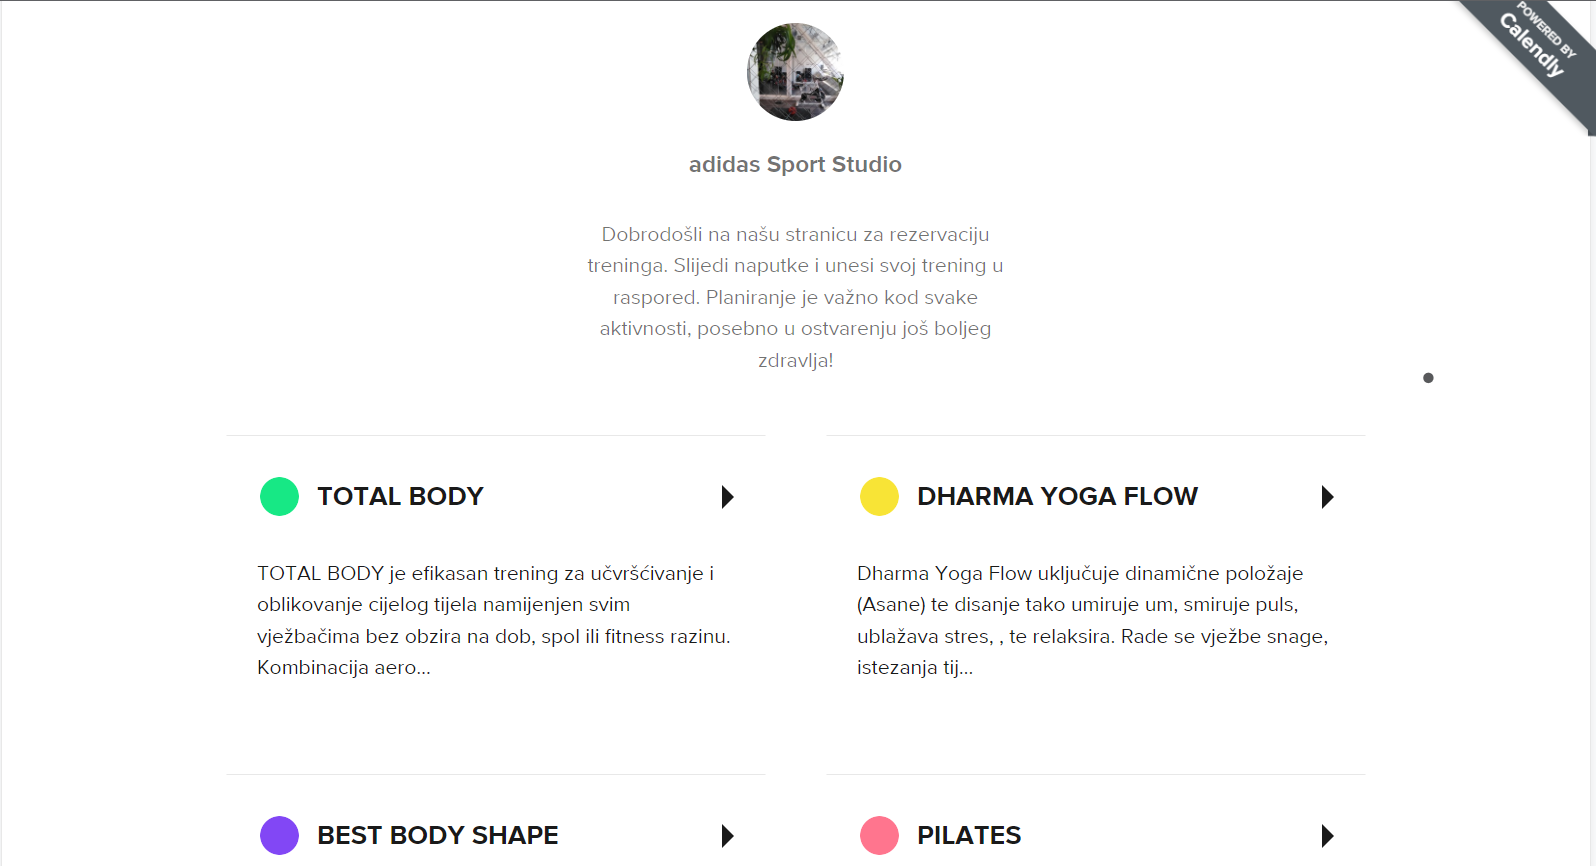
\includegraphics[scale=0.3]{slike/adidassportsstudio1.PNG} %veličina slike u odnosu na originalnu datoteku i pozicija slike
			\centering
			\caption{"Adidas Sports Studio" web aplikacija}
			\label{fig:adidassportsstudio1}
		\end{figure}
		
		\begin{figure}[H]
			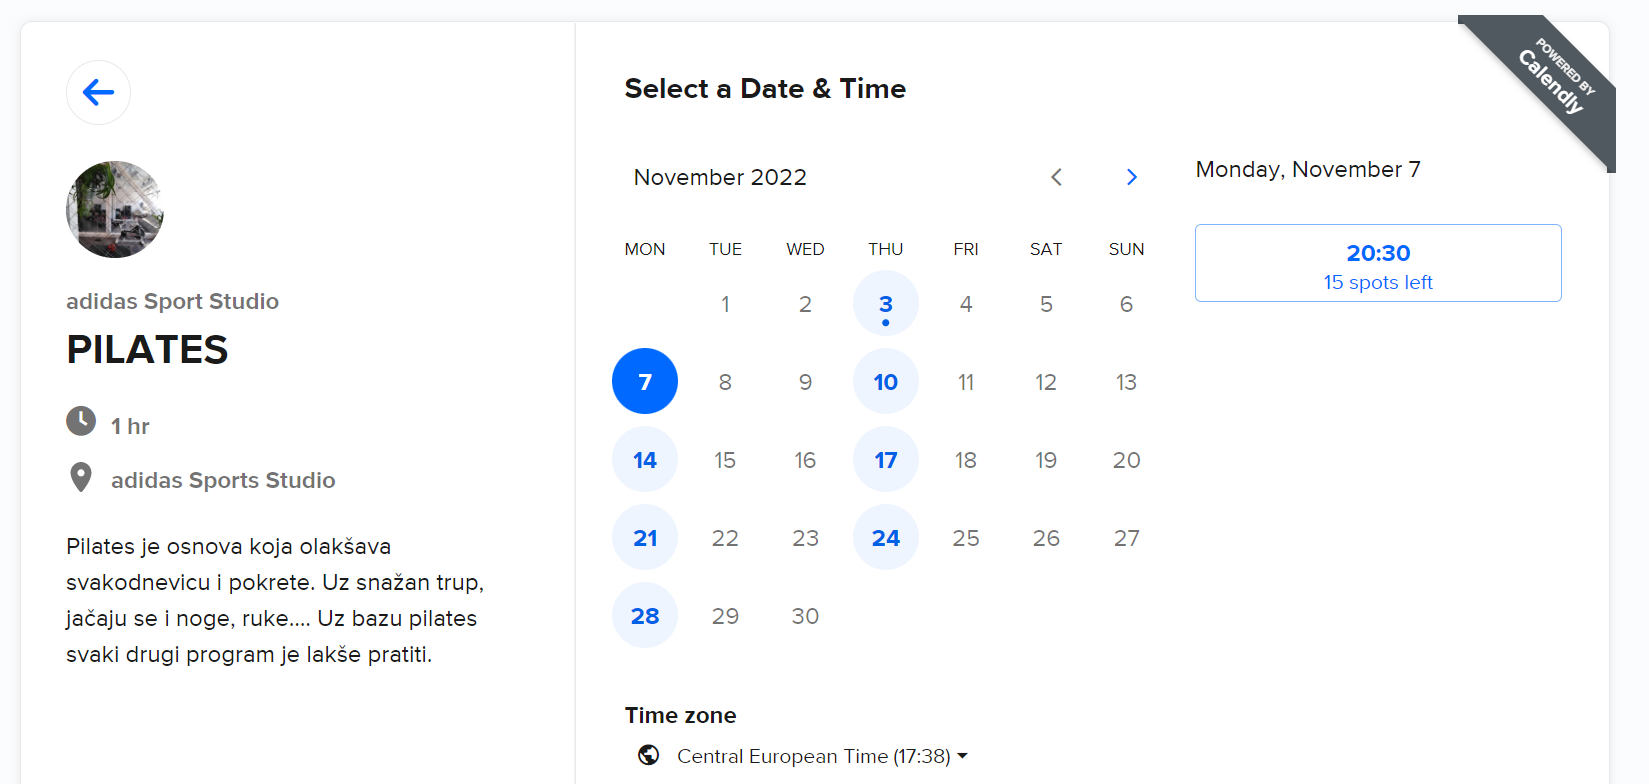
\includegraphics[scale=0.3]{slike/adidassportsstudio2.PNG} %veličina slike u odnosu na originalnu datoteku i pozicija slike
			\centering
			\caption{"Adidas Sports Studio" web aplikacija}
			\label{fig:adidassportsstudio2}
		\end{figure}
		
		\begin{figure}[H]
			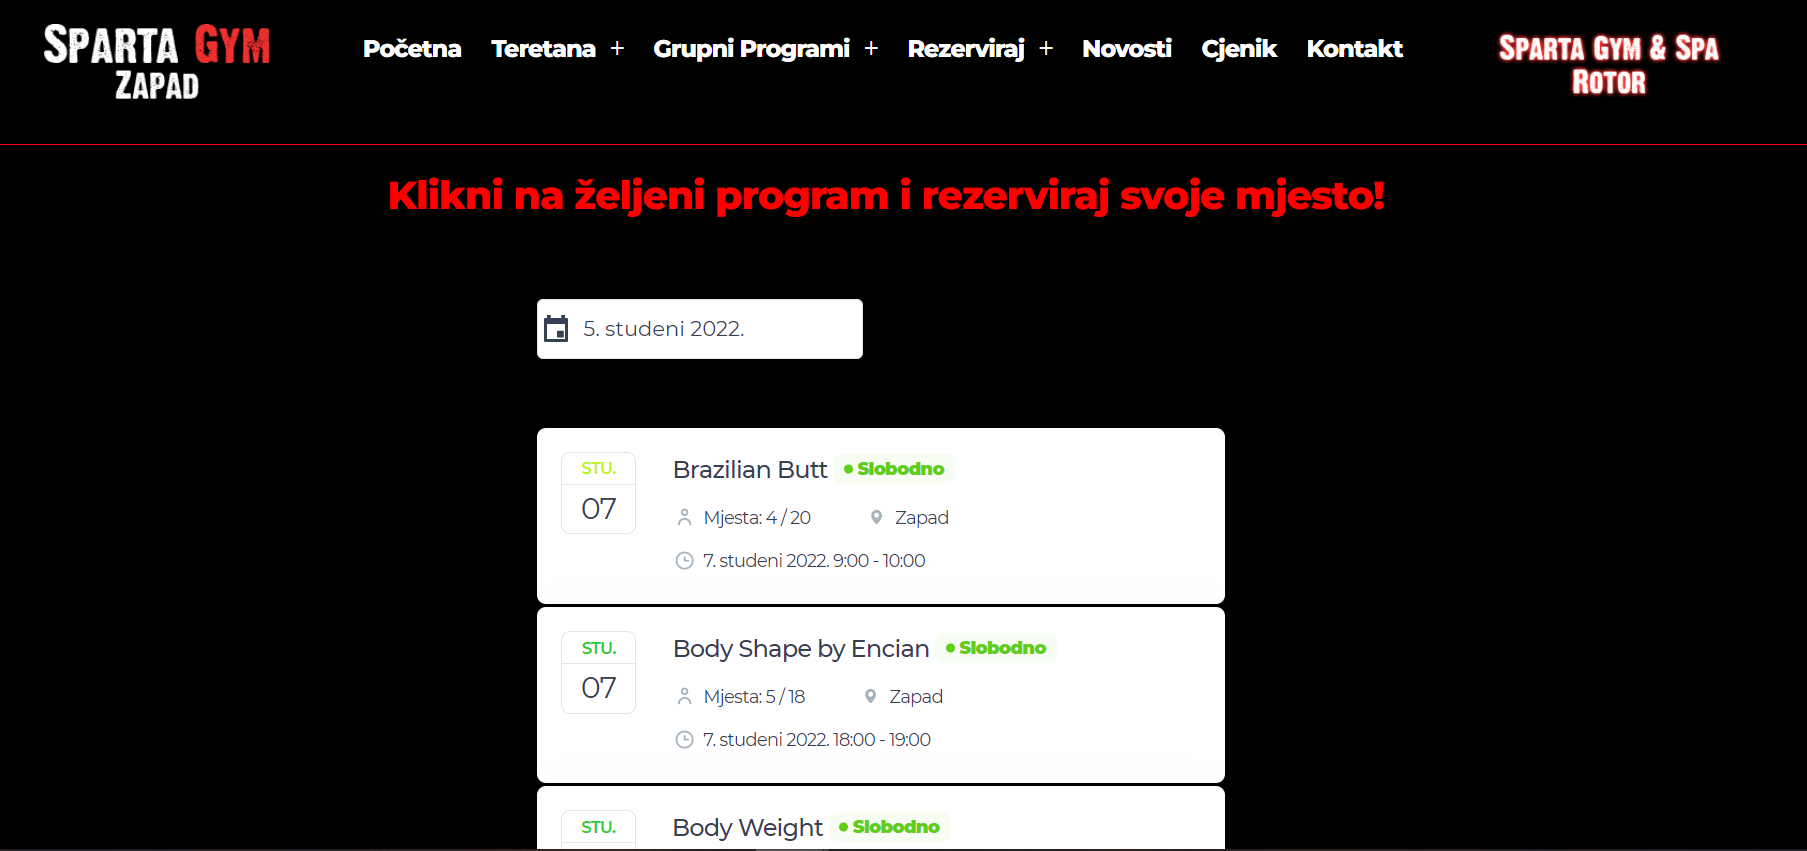
\includegraphics[scale=0.3]{slike/spartagym1.PNG} %veličina slike u odnosu na originalnu datoteku i pozicija slike
			\centering
			\caption{"Sparta Gym" web aplikacija}
			\label{fig:spartagym1}
		\end{figure}
		
		{Upravo zbog tog personaliziranog pristupa, smatramo da će aplikacija biti korisna svima onima koji nemaju vremena istražiti i inforimirati se o tome koje vrste vježbi bi najviše odgovarale njihovim potrebama.} 
		
		{Također, postoji puno prostora za nadogradnju aplikacije. jedan primjer je povezivanje nekoliko sportskih objekata u aplikaciji. Veliki broj tvrtki svojim zaposlenicima nudi korištenje "Multisport" kartice. To je kartica kojom je omogućen pristup velikom broju sportskih objekata u cijeloj Hrvatskoj. Tako bi aplikacija mogla nuditi termine treninga u različitim teretanama i sportskim prostorima. Time bi korisnici koji često putuju mogli rezervirati termine i u drugim gradovima te tako biti još redovitiji u pohađanju treninga. Drugi je primjer proširenja aplikacije da se uz tenere, uključe i stručnjaci na nekim drugim područjima osim fitnessa. Jedan primjer su nutricionisti. Ovisno o ciljevima koje korisnik odabire, nutricionist mu preporuča prehrambene namirnice koje bi bilo poželjno da uvrsti u vlastitu prehranu. Korisniku bi se tako uz termine treninga u kalendaru prikazivao i  jelovnik koji uključuje obroke koji sadrže preporučene namirnice. }
		
		
		\eject
		
	
	\chapter{Specifikacija programske potpore}
		
	\section{Funkcionalni zahtjevi}
			
			
			\noindent \textbf{Dionici:}
			
			\begin{packed_enum}

				 \item Korisnici treninga
				 \item Treneri
			     \item Administrator
			     \item Neregistrirani korisnici

				
			\end{packed_enum}
			
			\noindent \textbf{Aktori i njihovi funkcionalni zahtjevi:}
			
			
			\begin{packed_enum}


				\item  \underbar{Neregistrirani/neprijavljeni korisnik (inicijator) može:}
				
				\begin{packed_enum}
					
					\item registrirati se
					\item gumbom izbrisati sve unesene podatke pri registraciji
					\item prijaviti se
					\item pregledati početnu stranicu aplkacije
										
				\end{packed_enum}
			
				\item  \underbar{Korisnik treninga (inicijator) može:}
				
				\begin{packed_enum}
					
					\item prijaviti se u sustav korisničkim imenom i lozinkom
					\item pregledavati i mijenjati svoje osobne podatke (lozinku)
					\item vidjeti kroz kalendar kojim treninzima može prisustvovati ovisno o vježbama koje mora odrađivati
					\item rezervirati treninge na koje želi ići ovisno o fondu sati kojeg ima
					\item otkazati rezervaciju treninga
					
				\end{packed_enum}
			
			    \item  \underbar{Trener (inicijator) može:}
			    
			    \begin{packed_enum}
			    	
			    	\item prijaviti se u sustav koristeći ime i lozinku
			    	\item pregledavati sve registrirane korisničke račune
			    	\item odabrati registriranog korisnika treninga kojem može dodijeliti vježbe ovisno o ciljevima osobe
			    	\item stvarati treninge na mjesečnoj bazi (definirati vježbe i maksimalan broj polaznika) te ih unositi u kalendar
 			    	\item upisuje pravila o rezervaciji
			    	
			    \end{packed_enum}
		       
		        \item  \underbar{Administrator (inicijator) može:}
		        
		        \begin{packed_enum}
		        	
		        	\item prijaviti se
		        	\item administrirati korisničke račune te račune trenera
		        	\item ažurirati sve podatke u aplikaciji
		        	\item registrirati trenere
		        	
		        \end{packed_enum}

			\end{packed_enum}
			
			\eject 
			
			
				
			\subsection{Obrasci uporabe}
				
				
				\subsubsection{Opis obrazaca uporabe}
					

					\noindent \underbar{\textbf {UC1-Registracija}}				\begin{packed_item}
	
						\item \textbf{Glavni sudionik: }Neregistrirani korisnik treninga
						\item  \textbf{Cilj:} Stvoriti korisnički račun
						\item  \textbf{Sudionici:} Baza podataka
						\item  \textbf{Preduvjet:} UC15
						\item  \textbf{Opis osnovnog tijeka:}
						
						 \begin{packed_enum}
                      
	                        \item Neregistrirani korisnik odabire akciju "Registration" na početnoj stranici
	                        \item Sustav otvara formu za upis podataka
							\item Neregistrirani korisnik upisuje potrebne podatke (ime, prezime, koriničko ime, email, lozinku i ciljeve)
							\item Neregistrirani korisnik odabire opciju "Submit" 
							\item Sustav provjerava ispravnost unesenih podataka, sprema ih u bazu, prijavljuje korisnika, postavlja vrijeme isteka sesije na 30 minuta i otvara stranicu s osobnim podacima
							
						
						\end{packed_enum}
						
						\item*  \textbf{Opis mogućih odstupanja:}
						cx 5 m+cij9 jij66 +
						 \begin{packed_enum}
						 	\item[4.a] Neregistrirani korisnik odabire akciju Reset, a sustav na formi registracije briše sve unesene podatke. Sustav nastavlja izvođenje scenarija u koraku 3.
							\item[5.a] Sustav provjerava i utvrđuje da uneseni podaci nisu ispravni. Obavještava korisnika odgovarajućom porukom te nastavlja izvođenje scenarija u koraku 3 
							

								
						  \end{packed_enum}
						
					\end{packed_item}
				
				\noindent \underbar{\textbf {UC2-Prijava}}				\begin{packed_item}
						
						\item \textbf{Glavni sudionik: }Korisnik treninga, trener, administrator
						\item  \textbf{Cilj:} Prijaviti se u aplikaciju
						\item  \textbf{Sudionici:} Baza podataka
						\item  \textbf{Preduvjet:} UC15
						\item  \textbf{Opis osnovnog tijeka:}
						
						\item \begin{packed_enum}

							\item  Neprijavljeni korisnik odabire akciju "Log in" na početnoj stranici
							\item Sustav otvara formu za upis podataka
							\item Neprijavljeni korisnik upisuje potrebne podatke u formu (korisničko ime i lozinku)
							\item Sustav provjerava ispravnost podataka, prijavljuje korisnika, postavlja vrijeme isteka sesije na 30 minuta i otvara stranicu s osobnim podacima

							
						\end{packed_enum}
						
						\item  \textbf{Opis mogućih odstupanja:}
						
						\begin{packed_enum}
							
							\item[1.a] Ako neprijavljeni korisnik nema račun može izabrati akciju "Nemaš račun?" te sustav otvara formu za Registraciju
							\item[3.a] Sustav provjerava i utvrđuje da uneseni podaci nisu ispravni. Obavještava korisnika odgovarajućom porukom te nastavlja izvođenje scenarija u koraku 2
							
						\end{packed_enum}
						
					\end{packed_item}
				   
				\noindent \underbar{\textbf {UC3-Pregled osobnih podataka}}	\begin{packed_item}
						
						\item \textbf{Glavni sudionik: }Korisnik treninga, trener, administrator

						\item  \textbf{Cilj:} Pregled osobnih podataka

						\item  \textbf{Sudionici:} Baza podataka
						\item  \textbf{Preduvjet:} UC2
						\item  \textbf{Opis osnovnog tijeka:}
						
						\item[] \begin{packed_enum}
							
							\item Sustav prijavljenog korisnik nakon prijave/registracije automatski odvodi na stranicu osobnih podataka ili prijavljeni korisnik odabire akciju "Moji podaci" u zaglavlju aplikacije
							\item Korisnik ima uvid u svoje podatke (ime, prezime, koriničko ime, email, avatar)

							
						\end{packed_enum}
						
						\item  \textbf{Opis mogućih odstupanja:}
						
						\begin{packed_enum}
							
							\item /
							
						\end{packed_enum}
						
					\end{packed_item}
				
				\noindent \underbar{\textbf {UC4-Promjena osobnih podataka}}				\begin{packed_item}
						
						\item \textbf{Glavni sudionik: }Korisnik treninga
						\item  \textbf{Cilj:} Promjena svojih osobnih podataka
						\item  \textbf{Sudionici:} Baza podataka
						\item  \textbf{Preduvjet:} UC3
						\item  \textbf{Opis osnovnog tijeka:}
						
						\item[] \begin{packed_enum}

							
							\item Korisnik odabire akciju "Izmijeni"
							\item Sustav otvara formu za izmjenu lozinke
							\item Korisnik Nakon promjene odabire akciju "Save changes" 
							\item Sustav provjerava ispravnost podataka, sprema nove podatke u bazu i otvara stranicu s osobnim podacima

							
						\end{packed_enum}
						
						\item  \textbf{Opis mogućih odstupanja:}
						
						\begin{packed_enum}
							
							\item[4.a] Ako je korisnik mijenjao lozinku, sustav provjerava i utvrđuje da unesena stara lozinka nije ispravna. Obavještava korisnika odgovarajućom porukom te nastavlja izvođenje scenarija u koraku 2
							
						\end{packed_enum}
						
					\end{packed_item}
				
				
				\noindent \underbar{\textbf {UC5-Odabir ciljeva}}				\begin{packed_item}
						
						\item \textbf{Glavni sudionik: }Korisnik treninga
						\item  \textbf{Cilj:} Odabir ciljeva za taj mjesec
						\item  \textbf{Sudionici:} Baza podataka, trener
						\item  \textbf{Preduvjet:} UC3  
						\item  \textbf{Opis osnovnog tijeka:}
						
						\item[] \begin{packed_enum}

							\item Korisnik na stranici osobnih podataka iz padajućih izbornika odabire ciljeve
							\item Korisnik odabire akciju "Promijeni ciljeve"
							\item Sustav provjerava ima li korisnik pravo na promjenu ciljeva, mijenja ciljeve u bazi i otvara ponovno stranicu osobnih podataka

							
						\end{packed_enum}
						
						\item  \textbf{Opis mogućih odstupanja:}
						
						\begin{packed_enum}
							
							\item[1.a] Sustav je pri prijavi utvrdio da je korisnik taj mjesec već promijenio ciljeve i onemogućuje padajuće izbornike i gumb "Promijeni ciljeve".
							
						\end{packed_enum}
						
					\end{packed_item}
				
					\noindent \underbar{\textbf {UC6-Pregled termina treninga}}		
						\begin{packed_item}
						
						
						\item \textbf{Glavni sudionik: }Korisnik treninga
						\item  \textbf{Cilj:} Pregled datuma treninga
						\item  \textbf{Sudionici:} Baza podataka
						\item  \textbf{Preduvjet:} UC2
						\item  \textbf{Opis osnovnog tijeka:}
						
						\item[] \begin{packed_enum}
							
							\item Korisnik odabire akciju "Rezervacije" u zaglavlju aplikacije 
							\item Sustav otvara kalendar s terminima treninga koje taj korisnik može rezervirati i naznačenim preostalim satima
							\item Korisnik odabire jedan od dostupnih treninga 
							\item Susatv prikazuje u popup prozoru detalje o terminu (vrijeme početka, vrijeme kraja, ime i prezime trenera, listu vježbi i broj preostalih mjesta)

							
						\end{packed_enum}
						
						\item  \textbf{Opis mogućih odstupanja:}
						
						\begin{packed_enum}
							
							\item[3.a] Sustav utvrđuje da korisniku nisu dodijeljene vježbe pa time ni treninzi te obavještava korisnika porukom na sredini ekrana.
							
						\end{packed_enum}
						
					\end{packed_item}
				
				
					\noindent \underbar{\textbf {UC7-Rezervacija termina treninga}}		
						\begin{packed_item}
						
						\item \textbf{Glavni sudionik: }Korisnik treninga
						\item  \textbf{Cilj:}Rezervacija termina
						\item  \textbf{Sudionici:} Baza podataka
						\item  \textbf{Preduvjet:} UC6
						\item  \textbf{Opis osnovnog tijeka:}
						
						\item[] \begin{packed_enum}

							\item Korisnik nakon odabira treninga odabire akciju "Reserve" 
							\item Sustav provjerava fond sati, smanjuje ih za 1, sprema podatke za korisnika i termin u bazu te otvara stranicu Rezervacije
							\item Sustav rezrviranom treningu nadodaje akciju "Cancel reservation"

							
						\end{packed_enum}
						
						\item  \textbf{Opis mogućih odstupanja:}
						
						\begin{packed_enum}
							
							\item[1.a] Sustav utvrđuje da u terminu nema više slobodnih mjesta te onemogućuje gumb Reserve za taj termin
							\item[1.b] Sustav utvrđuje da korisnik nema više preostalih sati, onemogućuje gumb Reserve i obavještava korisnika porukom iznad kalendara
							
						\end{packed_enum}
						
					\end{packed_item}
				
				
					\noindent \underbar{\textbf {UC8-Pregled datuma treninga i termina po danu 2}}				\begin{packed_item}
						
						\item \textbf{Glavni sudionik: }Trener
						\item  \textbf{Cilj:} Pregled datuma treninga 
						\item  \textbf{Sudionici:} Baza podataka
						\item  \textbf{Preduvjet:} UC2
						\item  \textbf{Opis osnovnog tijeka:}
						
						\item[] \begin{packed_enum}
							
							\item Trener odabire akciju "Termini" u zaglavlju aplikacije 
							\item Sustav otvara kalendar sa svim terminima drugih trenera i njegovim, posebno obojanim, terminima treninga.
							\item Trener odabire jedan od termina 
							\item Susatv prikazuje u popup prozoru detalje o terminu (vrijeme početka, vrijeme kraja, ime i prezime trenera, listu vježbi i broj preostalih mjesta)

							
						\end{packed_enum}
						
						\item  \textbf{Opis mogućih odstupanja:}
						
						\begin{packed_enum}
							
							\item /
							
						\end{packed_enum}
						
					\end{packed_item}
				
					\noindent \underbar{\textbf {UC9-Unos treninga}}			\begin{packed_item}
						
						\item \textbf{Glavni sudionik: }Trener
						\item  \textbf{Cilj:} Unos novog termina
						\item  \textbf{Sudionici:} Baza podataka
						\item  \textbf{Preduvjet:} UC2
						\item  \textbf{Opis osnovnog tijeka:}
						
						\item[] \begin{packed_enum}
							
							\item Trener odabire akciju "Termini" u zaglavlju aplikacije 
							\item Sustav otvara kalendar sa svim terminima drugih trenera i njegovim, posebno obojanim, terminima treninga.
							\item Trener odabire akciju dodaj termin
							\item Sustav otvara formu za unos podataka
							\item Trener unosi podatke (vrijeme početka treninga, vrijeme kraja, vrstu treninga i broj mjesta) i odabire akciju "Create"
							\item Sustav provjerava unesene podatke, sprema ih u bazu i otvara kalendar s terminima
							
							
						\end{packed_enum}
						
						\item  \textbf{Opis mogućih odstupanja:}
						
						\begin{packed_enum}
							
							\item[6.a] Sustav utvrđuje da postoji preklapanje između tog termina i već postojećeg ili da je prevelik broj polaznika te obavjestava korisnika odgovarajućom porukom i anstavlja izvodenje od koraka 4
							
						\end{packed_enum}
						
					\end{packed_item}
					
					
				   	\noindent \underbar{\textbf {UC10-Pregled liste registriranih korisnika}}
				   		
				   				
				   		\begin{packed_item}
				   		
				   		\item \textbf{Glavni sudionik: }Trener
				   		\item  \textbf{Cilj:}Pregled korisnika treninga
				   		\item  \textbf{Sudionici:} Baza podataka
				   		\item  \textbf{Preduvjet:} UC2
				   		\item  \textbf{Opis osnovnog tijeka:}
				   		
				   		\item[] \begin{packed_enum}
				   			
				   			\item Trener odabire akciju "Korisnici" u zaglavlju aplikacije
				   			\item Sustav otvara stranicu s listom registriranih korisnika treninga, oni bez dodijeljenih vježbi su obojani drugačije i imaju uz sebe gumb "Dodijeli vježbu"
				   			
				   		\end{packed_enum}
				   		
				   		\item  \textbf{Opis mogućih odstupanja:}
				   		
				   		\begin{packed_enum}
				   			
				   			\item[2.a]Sustav utvrđuje da nema registriranih korisnika te obavještava trenera odgovarajućom porukom
				   			
				   		\end{packed_enum}
				   		
				   	\end{packed_item}
			   	
			   	\noindent \underbar{\textbf {UC11-Dodjela vježbi}}	
			   		
			   		
			   		\begin{packed_item}
			   			
			   			\item \textbf{Glavni sudionik: }Trener
			   			\item  \textbf{Cilj:}Dodjela vježbi korisniku treninga shodno njihovom cilju
			   			\item  \textbf{Sudionici:} Baza podataka, usluga e-pošte
			   			\item  \textbf{Preduvjet:} UC10
			   			\item  \textbf{Opis osnovnog tijeka:}
			   			
			   			\item[] \begin{packed_enum}
			   				
			   				\item Trener odabire akciju "Dodijeli vježbe"
			   				\item Sustav otvara popup prozor s opisom ciljeva tog korisnika i 3 padajuća izbornika za 3 vježbe
			   				\item Trener bira vježbe i odabire akciju "Save"
			   				\item Sustav provjerava vježbe, sprema ih u bazu i otvara nanovo popis korisnika
			   				
			   				
			   			\end{packed_enum}
			   			
			   			\item  \textbf{Opis mogućih odstupanja:}
			   			
			   			\begin{packed_enum}
			   				
			   				\item[4.a] Sustav utvrđuje da je trener odabrao više istih vježbi, obavještava ga porukom i nastavlja od koraka 2
			   				
			   			\end{packed_enum}
			   			
			   		\end{packed_item}
		   		
		   			\noindent \underbar{\textbf {UC12-Brisanje termina treninga 3}}
		   			
		   			
		   			\begin{packed_item}
		   				
		   				\item \textbf{Glavni sudionik: }Administrator
		   				\item  \textbf{Cilj:} Pregled termina
		   				\item  \textbf{Sudionici:} Baza podataka
		   				\item  \textbf{Preduvjet:} UC2
		   				\item  \textbf{Opis osnovnog tijeka:}
		   				
		   				\item[] \begin{packed_enum}
		   					
		   					\item Administrator odabire akciju "Termini" u zaglavlju aplikacije
		   					\item Sustav otvara stranicu s kalendarom sa svim postojećim terminima treninga
		   					\item Administrator odabire termin te odabire opciju "Delete"
		   					\item Sustav briše termin iz baze podataka i otvara nanovo kalendar s terminima
		   					
		   				\end{packed_enum}
		   				
		   				\item  \textbf{Opis mogućih odstupanja:}
		   				
		   				\begin{packed_enum}
		   					
		   					\item /
		   					
		   				\end{packed_enum}
		   				
		   			\end{packed_item}
	   			
	   			
	   				\noindent \underbar{\textbf {UC13-Registracija trenera}}
	   				
	   				
	   				\begin{packed_item}
	   					
	   					\item \textbf{Glavni sudionik: }Administrator
	   					\item  \textbf{Cilj:} Registracija trenera
	   					\item  \textbf{Sudionici:} Baza podataka
	   					\item  \textbf{Preduvjet:} UC2
	   					\item  \textbf{Opis osnovnog tijeka:}
	   					
	   					\item[] \begin{packed_enum}
	   						
	   						\item Administrator odabire akciju "Register Trainer" u zaglavlju aplikacije
	   						\item Sustav otvara formom za upis podataka o novom treneru (ime, prezime, korisničko ime, lozinka, email)
	   						\item Administrator upisuje podatke i odabire akciju "Register"
	   						\item Sustav provjerava podatke sprema trenera u bazu i otvara početnu stranicu
	   						
	   						
	   					\end{packed_enum}
	   					
	   					\item  \textbf{Opis mogućih odstupanja:}
	   					
	   					\begin{packed_enum}
	   						
	   						\item[4.a] Sustav utvrđuje da su uneseni krivi podaci(npr. korisničko ime već postoji), obavještava administratora odgovarajućom porukom i nastavlja od koraka 2
	   						
	   					\end{packed_enum}
	   					
	   				\end{packed_item}
   				
   				\noindent \underbar{\textbf {UC14-Odjava}}
   				
   				
   				\begin{packed_item}
   					
   					\item \textbf{Glavni sudionik: }Prijavljeni korisnik
   					\item  \textbf{Cilj:}Odjava s računa 
   					\item  \textbf{Sudionici:} Baza podataka
   					\item  \textbf{Preduvjet:} UC3
   					\item  \textbf{Opis osnovnog tijeka:}
   					
   					\item[] \begin{packed_enum}
   						
   						\item Korisnik odabire akciju "Log out" 
   						\item Sustav odjavljuje korisnika i otvara početnu stranicu
   						
   						
   					\end{packed_enum}
   					
   					\item  \textbf{Opis mogućih odstupanja:}
   					
   					\begin{packed_enum}
   						
   						\item /
   						
   					\end{packed_enum}
   					
   				\end{packed_item}
   			
   			    \noindent \underbar{\textbf {UC15-Pregled početne stranice}}
   			    
   			    
   			    \begin{packed_item}
   			    	
   			    	\item \textbf{Glavni sudionik: }Korisnik (bilo tko)
   			    	\item  \textbf{Cilj:}Pregled početne stranice aplikacije na kojoj pobliže opisujemo te reklamiramo našu aplikaciju koja koristi za upravljanje grupnih treninga 
   			    	\item  \textbf{Sudionici:} /
   			    	\item  \textbf{Preduvjet:} /
   			    	\item  \textbf{Opis osnovnog tijeka:}
   			    	
   			    	\item[] \begin{packed_enum}
   			    		
   			    		\item Upis adrese naše aplikacije u internet tražilicu
   			    		
   			    	\end{packed_enum}
   			    	
   			    	\item  \textbf{Opis mogućih odstupanja:}
   			    	
   			    	\begin{packed_enum}
   			    		
   			    		\item /
   			    		
   			    	\end{packed_enum}
   			    	
   			    \end{packed_item}
				\subsubsection{Dijagrami obrazaca uporabe}
					
						\begin{figure}[H]
						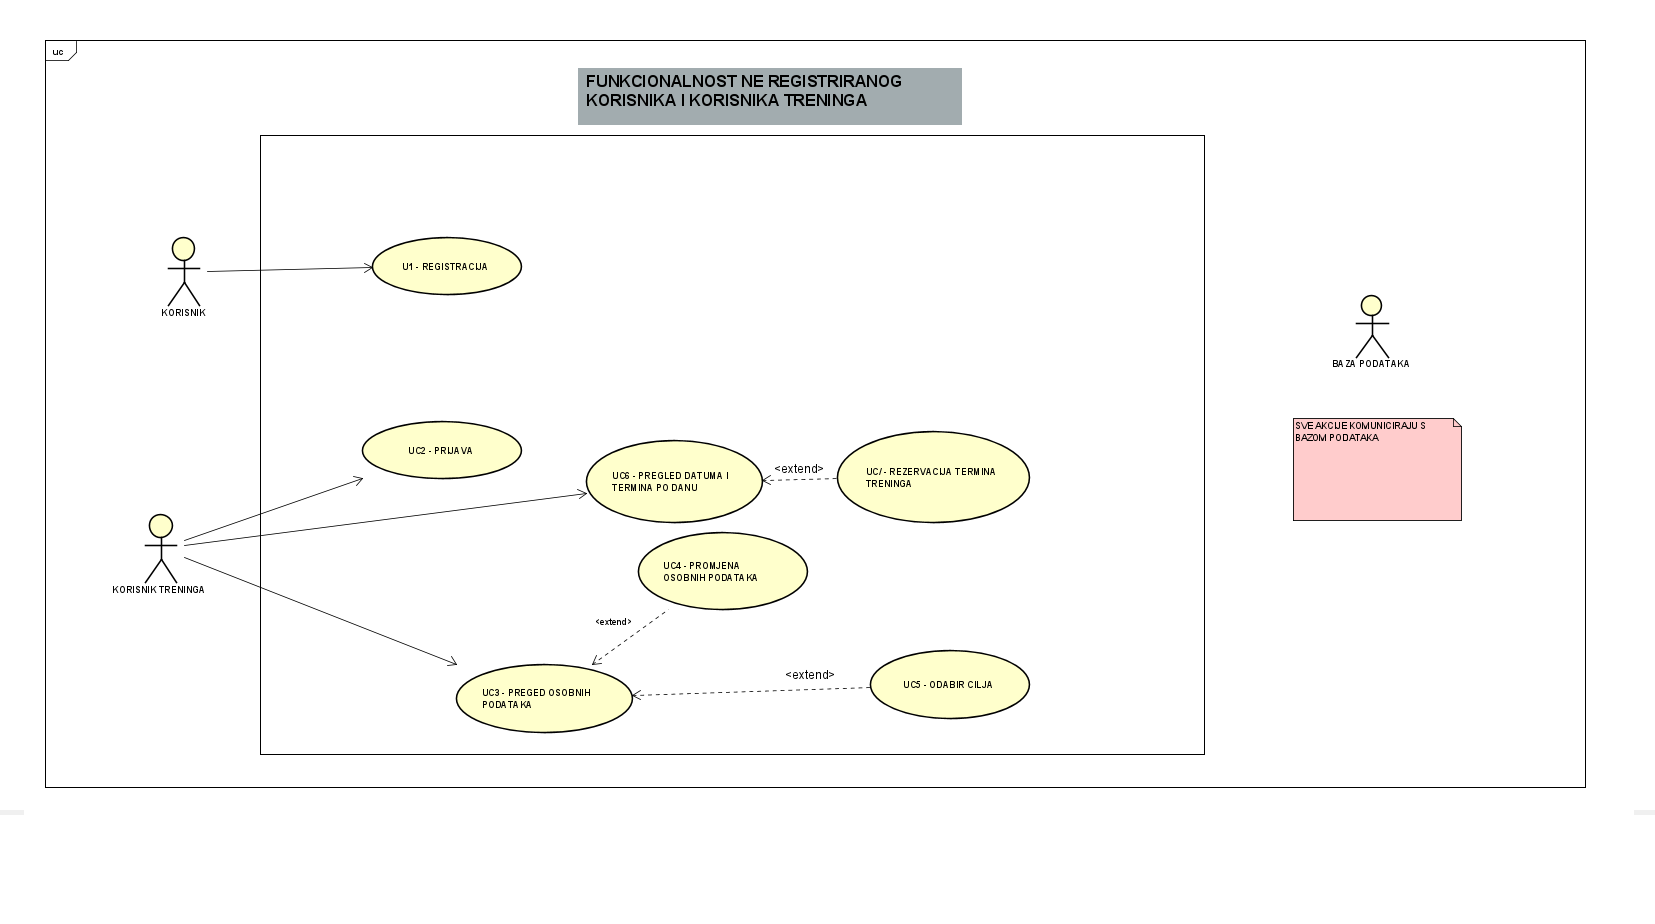
\includegraphics[scale=0.5]{dijagrami/nestodrugo.png} %veličina slike u odnosu na originalnu datoteku i pozicija slike
						\centering
						\caption{"Dijagram funckionalnosti neregistriranog korisnika i korisnika treninga"}
						\label{fig:ou1}
				     	\end{figure}
			     	
			     	\begin{figure}[H]
			     		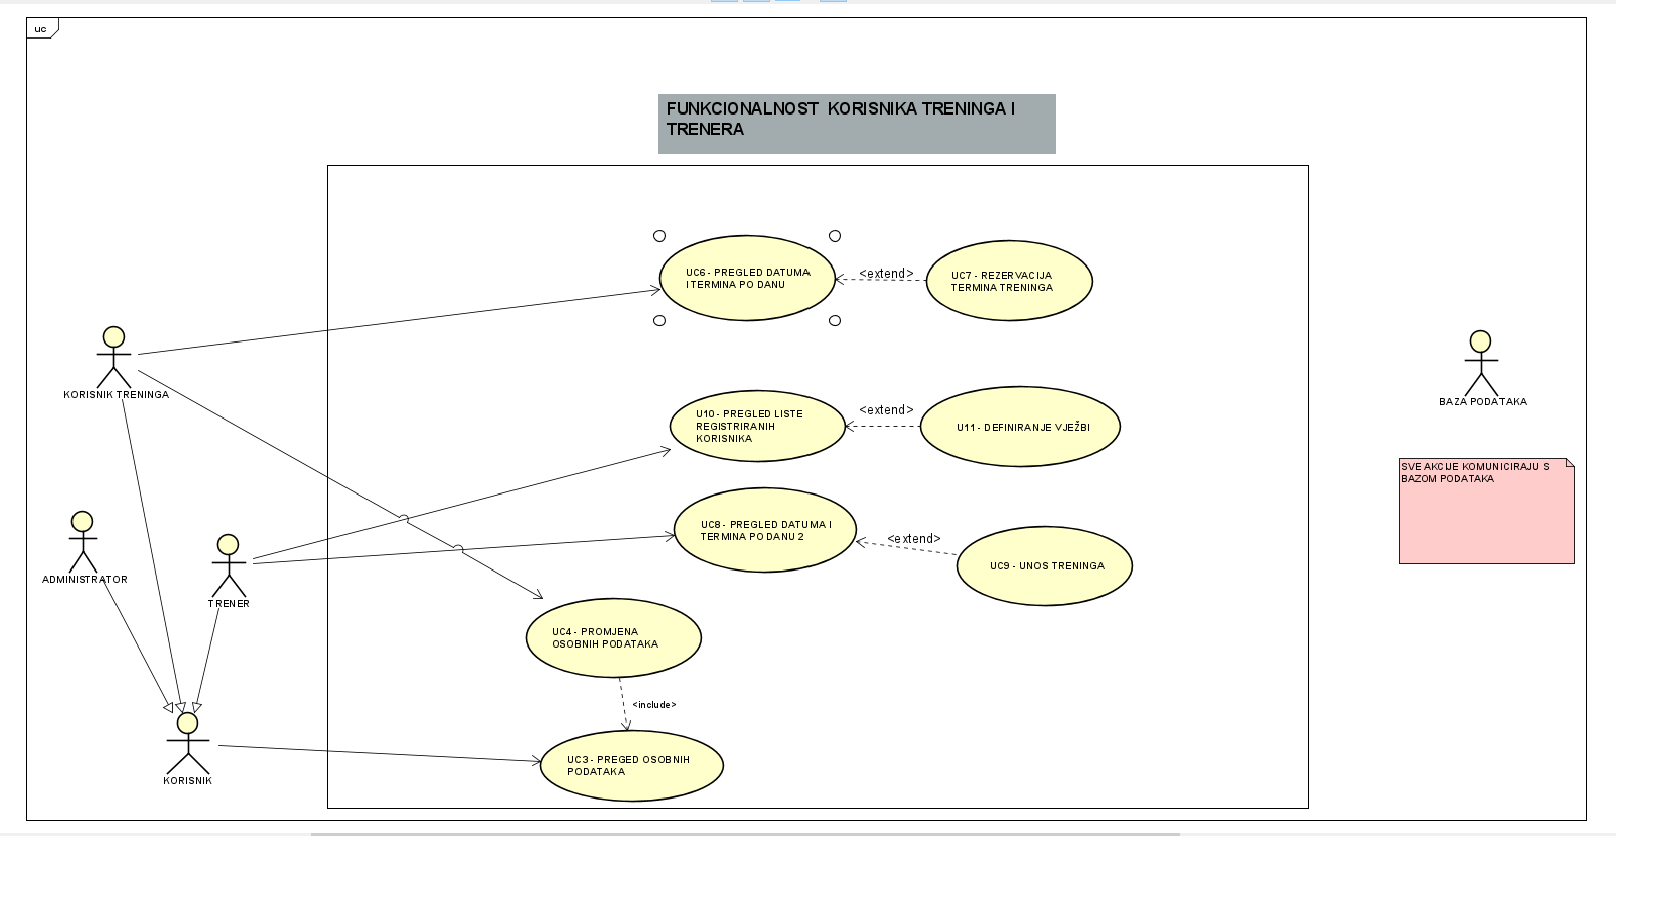
\includegraphics[scale=0.5]{dijagrami/drugidijagramou.png} %veličina slike u odnosu na originalnu datoteku i pozicija slike
			     		\centering
			     		\caption{"Dijagram funkcionalnosti korisnika treninga i trenera"}
			     		\label{fig:ou2}
			     	\end{figure}
		     	
		     	\begin{figure}[H]
		     		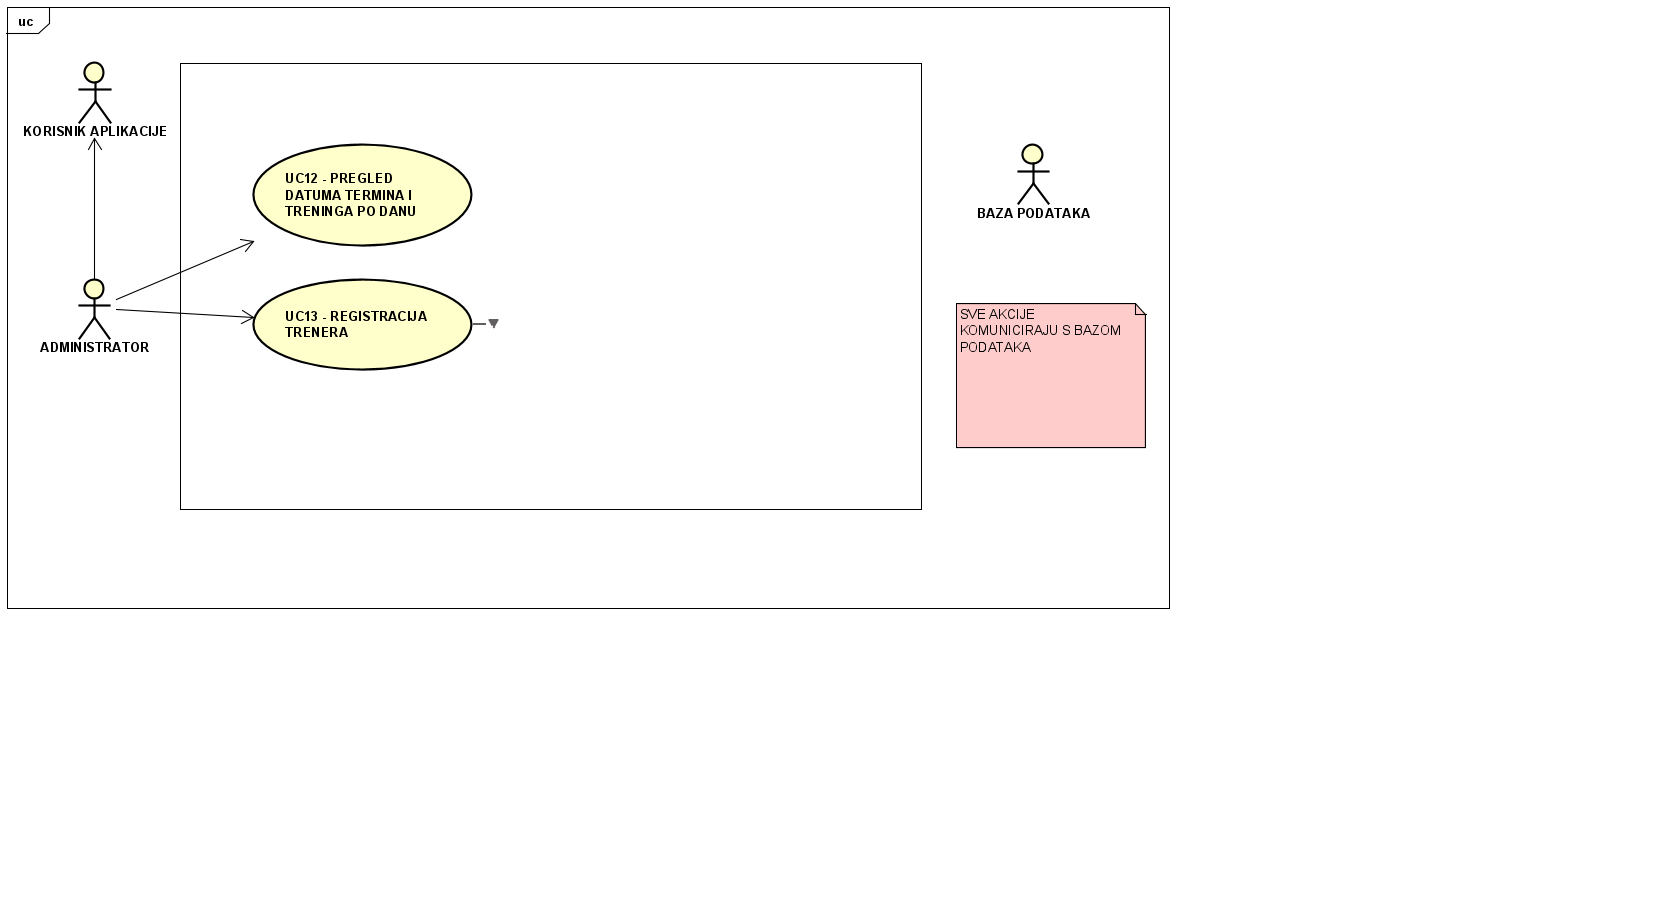
\includegraphics[scale=0.5]{dijagrami/trecidijagramou.png} %veličina slike u odnosu na originalnu datoteku i pozicija slike
		     		\centering
		     		\caption{"Dijagram funckionalnosti korisnika aplikacije i administratora"}
		     		\label{fig:ou3}
		     	\end{figure}
					
			\subsection{Sekvencijski dijagrami}
				
				

				\textbf{\textit{Obrazac uporabe UC1 - Registracija}}\\
	
				{Klijent šalje zahtjev za stranicu registracije kako bih se mogao registrirati. Poslužitelj dohvaća stranicu za registraciju te ju prikazuje. Zatim klijent ispunjava formu za registraciju te ju šalje poslužitelju. Poslužitelj provjerava ispravnost podataka te ukoliko su ispravni zapisuje podatke u bazu podataka. Nakon uspješne registracije poslužitelj klijentu prikazuje stranicu s osobnim podacima.
					
				
				\begin{figure}[H]
					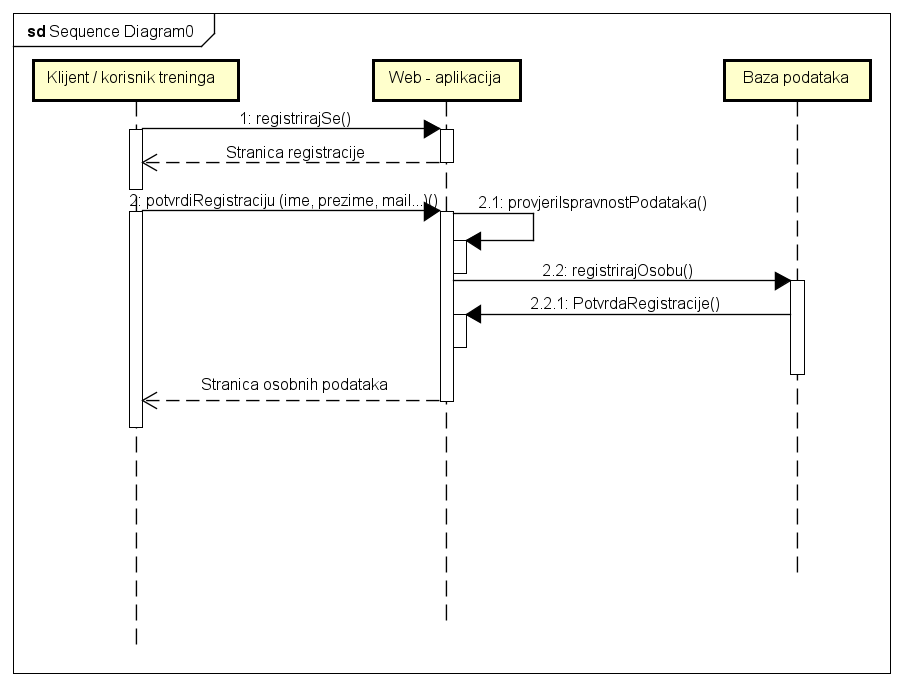
\includegraphics[scale=0.6]{dijagrami/sekvencijskiVukelic.png} %veličina slike u odnosu na originalnu datoteku i pozicija slike
					\centering
					\caption{"Registracija"}
					\label{fig:sekvencijski1}
				\end{figure}
			
				\eject
				
				\textbf{\textit{Obrazac uporabe UC7 - Rezervacija termina treninga}}\\
				
			
				{Klijent šale zahtjev za prikaz stranice za prijavu. Poslužitelj vraća stranicu za prijavu te klijent nastavlja s prijavom unoseći svoje podatke(username i password). Nakon unosa podataka poslužitelj provjerava ispravnost podataka sa bazom podataka te ukoliko je uspješno poslužitelj klijentu prikazuje stranicu kalendara. Zatim klijent bira željene termine te poslužitelj provjerava u bazi podataka ima li klijent dovoljno sati u vlastitom fondu. Ukoliko nema prikazuje se alert poruka u suprotnom poslužitelj sprema odabrane termine klijenta u bazu podataka te umanjuje preostali fond sati klijenta. Nakon obavljenih operacija poslužitelj klijentu prikazuje tipku "odustani" ukoliko klijent želi odustati od rezerviranih termina.}
				
				
				\begin{figure}[H]
					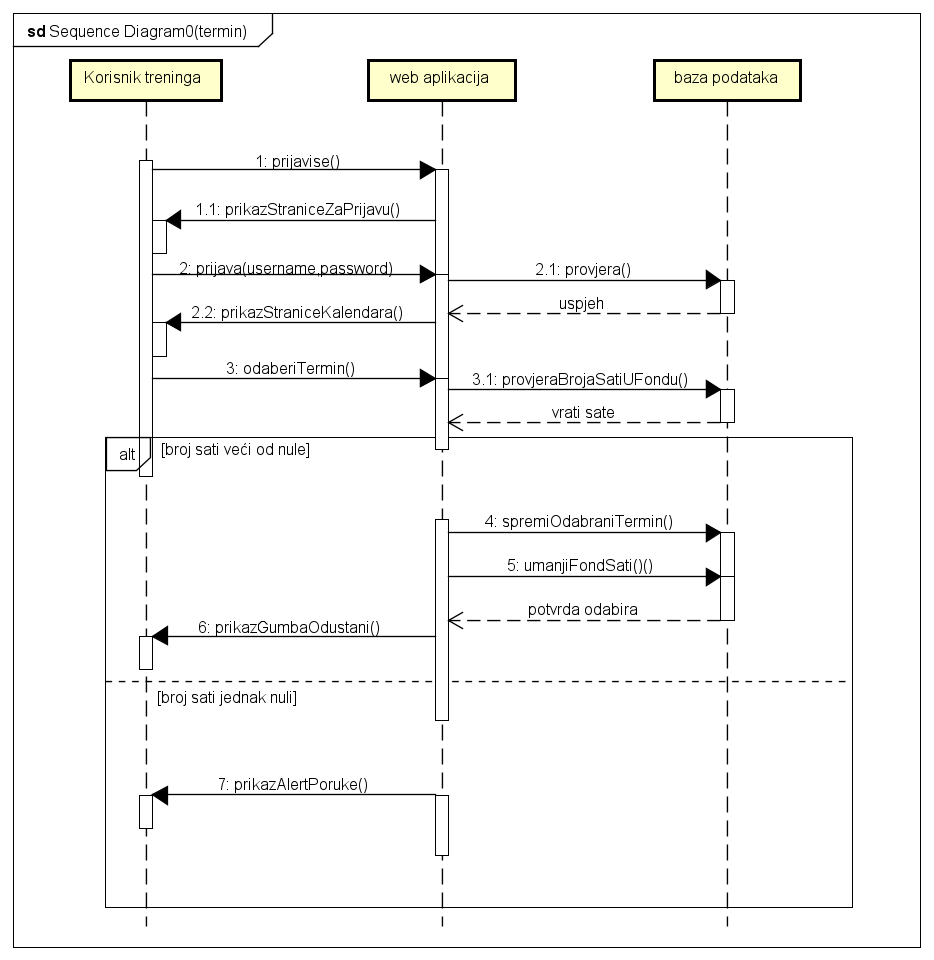
\includegraphics[scale=0.6]{dijagrami/UC7fixedsequental.png} %veličina slike u odnosu na originalnu datoteku i pozicija slike
					\centering
					\caption{"Rezervacija termina treninga"}
					\label{fig:sekvencijski2}
				\end{figure}
				
				\eject
				
				\textbf{\textit{Obrazac uporabe UC9 - Unos treninga}}\\
				
				
				{Klijent u ovom slučaju trener šalje zahtjev za prikaz stranice kalendara. Poslužitelj vraća stranicu kalendara te trener nastavlja s unosom termina treninga birajući na kalendaru u kojem terminu želi da se trening odvija. Nakon odabira termina poslužitelj sprema odabrani termin u bazu podataka zajedno s vježbama koje će se obavljati tokom treninga. Nakon spremanja u bazu podataka poslužitelj mjenja boju termina kako bih znali da je termin popunjen. }
				
				
				\begin{figure}[H]
					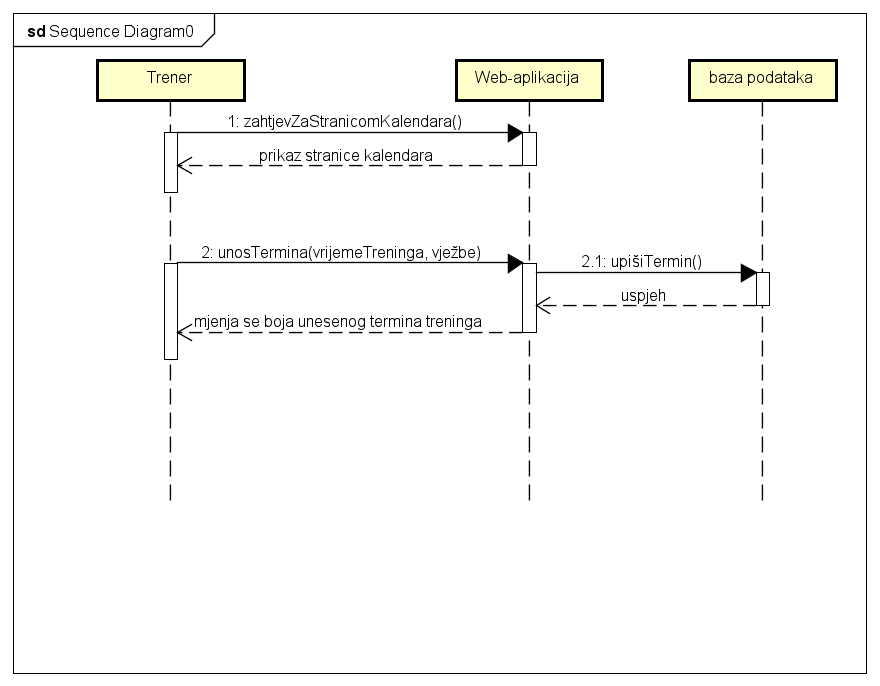
\includegraphics[scale=0.6]{dijagrami/UC9sekvencijski.png} %veličina slike u odnosu na originalnu datoteku i pozicija slike
					\centering
					\caption{"Unos treninga"}
					\label{fig:sekvencijski3}
				\end{figure}
				
				\eject
				
				\textbf{\textit{Obrazac uporabe UC14 - Odjava}}\\
				
				
				{Klijent zatraži od poslužitelja stranicu osobnih podataka. Poslužitelj vraća klijentu stranicu poslužitelja te zatim klijent klikne gumb "logout". Poslužitelj zatim odjavljenom korisniku prikazuje početnu stranicu web aplikacije.}
				
				
				\begin{figure}[H]
					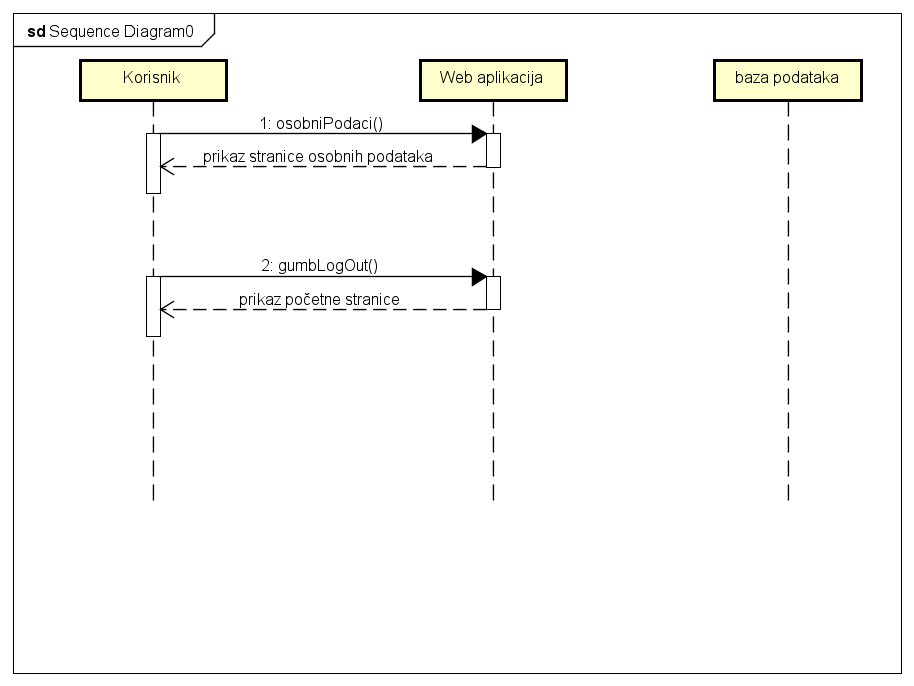
\includegraphics[scale=0.6]{dijagrami/UC14.png} %veličina slike u odnosu na originalnu datoteku i pozicija slike
					\centering
					\caption{"Odjava"}
					\label{fig:sekvencijski4}
				\end{figure}
				
				\eject

		\section{Ostali zahtjevi}
			 
			 \begin{packed_item}
			 	\item { Aplikacija treba biti izvedena kao web aplikacija kojoj će korisnici pristupati uz pomoć korisničkog imena i lozinke}
			 	\item {Aplikacija treba biti jednostavna za korištenje, a sučelje pregledno i intuitivno}
			 	\item {Aplikacija treba biti prilagođena za rad na različitim uređajima (mobilni uređaj, tablet, PC)}
			 	\item {Aplikacija mora osigurati sigurnost baze podataka i otpornost na vanjske prijetnje}
			 	\item {Aplikacija mora omogućiti rad više korisnika istovremeno}
			 	\item {Korisničko sučelje treba podržavati englesku abecedu pri unosu i prikazu sadržaja}
			 \end{packed_item}
			 
			 
			 
	
	\chapter{Arhitektura i dizajn sustava}
      
      {Arhitektura sustava naše aplikacije implementirana je u arhitekturi klijent-poslužitelj.}
       
      {Na klijentskoj strani koristili smo programski jezik \textit{JavaScript}, radni okvir \textit{React} i biblioteku komponenata \textit{Material UI} u uređivaču \textit{Visual Studio Code}.}
      
      {Na poslužiteljskoj strani koristili smo programski jezik \textit{Java} i radni okvir \textit{Spring Boot} u uređivaču \textit{IntelliJ IDEA}. Poslužiteljska strana organizirana je u tri sloja. To su nadglednik (controller), usluga (service) i repozitorij (repository). Nadglednik povezuje korisničku stranu s poslužiteljskom stranom. Sloj usluga ostvaruje temeljnu funkcionalnost web aplikacije i definira jednu ili više usluga web aplikacije. Repozitorij osigurava pristup podacima.}
      	
      {Podatke smo spremali u relacijsku bazu podataka \textit{PostgreSql} koristeći \textit{Java Persistence API}.} 
      
      
      \begin{figure}[H]
      	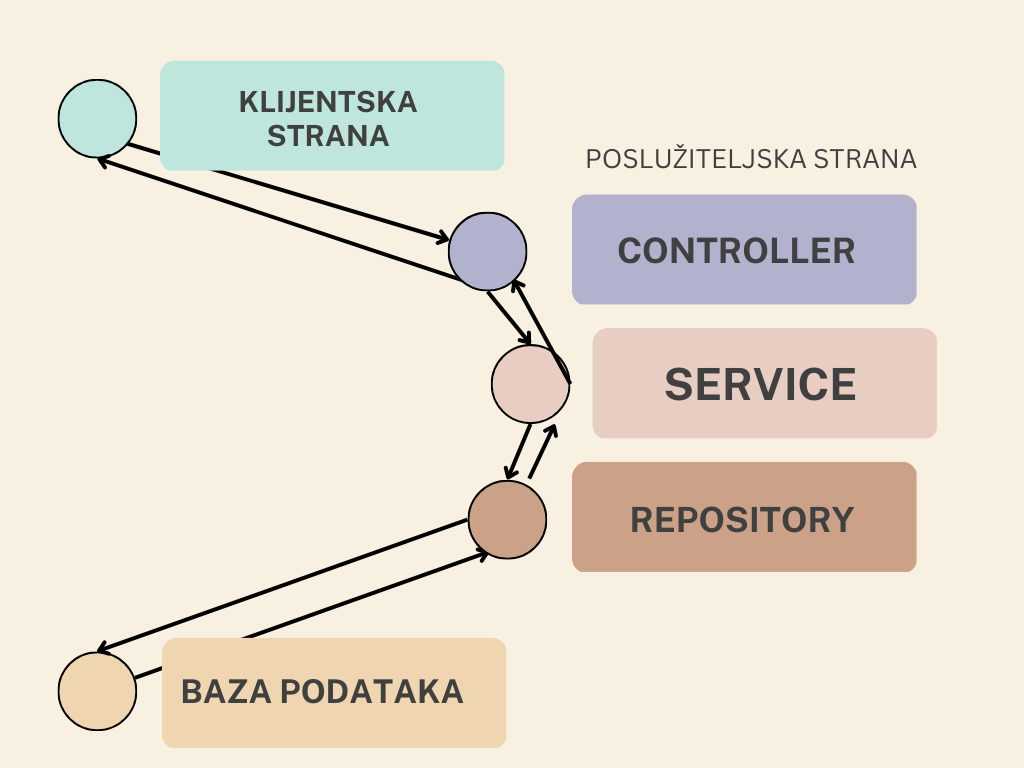
\includegraphics[scale=0.3]{slike/povezanostslojeva.PNG} %veličina slike u odnosu na originalnu datoteku i pozicija slike
      	\centering
      	\caption{Povezanost slojeva u radnom okviru Spring}
      	\label{fig:povezanostslojeva.png}
      \end{figure}
  
      {Osim toga postoji i razrađeni model podataka domene (domenski
      	objekti) kojeg koriste svi slojevi po potrebi. Razredi koji su sadržani u modelu domene imaju oznaku @Entity i sadrže podatke koji se
      	postavljaju i čitaju putem metoda get i set. Nadglednik koristi domenske objekte za automatsko postavljanje vrijednosti objekata iz tijela
      	zahtjeva (@RequestBody) od klijentske strane, sloj usluge korisit ih za ostvarenje odgovarajuće funkcionalnosti aplikacije, a repozitorij za automatskopreslikavanje objekta u relaciju u bazi podataka i obratno.}
      
      



				
		\section{Baza podataka}
		
		 {U implementaciji naše web aplikacije koristimo relacijsku bazu podataka. Objekti u relacijskoj bazi podataka su relacije, tj. dvodimenzionalne tablice koje su definirane imenom, a atributi su imenovani stupci relacije. Glavna zadaća baze podataka je pohrana, izmjena i dohvat podataka za daljnju obradu. Baza podataka ove aplikacije sastoji se od sljedećih entiteta: }
		  \begin{packed_item}
		  	\item {User}
		  	\item {Updates}
		  	\item {TrainingSession}
		  	\item {TrainingType}
		  	\item {Exercise}
		  	\item {Goal}
		  \end{packed_item}
		
			\subsection{Opis tablica}
			

				{Entitet \textbf {User} sadrži sve podatke o korisniku aplikacije.Sadrži atribute korisničko ime, ime korisnika, prezime, email adresu, lozinku, ulogu koju korisnik ima, prvi i drugi cilj, preostali broj termina treninga koje korisnik ima pravo rezervirati ovaj mjesec i novi cilj korisnika. Ovaj entitet u vezi je \textit{One-to-One} s entitetom \textit{Updates} preko atributa username i u vezi je s \textit{Many-to-One} s \textit{TrainingSession} preko atributa username.
				
				\begin{longtblr}[
					label=none,
					entry=none
					]{
						width = \textwidth,
						colspec={|X[11,l]|X[6, l]|X[20, l]|}, 
						rowhead = 1,
						cell{1}{1} = {c=3}{c},
					}
					\hline 
					\textbf{User} & & 	 \\ \hline[3pt]
					\SetCell{LightGreen}username & VARCHAR	&  	jedinstveno korisničko ime	\\ \hline
					firstName	& VARCHAR &   ime korisnika	\\ \hline 
					lastName & VARCHAR & prezime korisnika  \\ \hline 
					email & VARCHAR	&  	e-mail korisnika	\\ \hline 
					password & VARCHAR	&  	lozinka korisnika	\\ \hline
					role & VARCHAR	&  	uloga korisnika	\\ \hline
					goal1 & VARCHAR	&  	prvi cilj korisnika	\\ \hline 
					goal2 & VARCHAR	&  	drugi cilj korisnika	\\ \hline 
					remainingTrainingSessions & INT	&  	preostali termini korisnika \\ \hline
					newGoal & INT	&   novi cilj	\\ \hline 	 
				\end{longtblr}
			
			{Entitet \textbf{Updates} identifikacijski je slabi entitet koji ovisi o entitetu \textit{User}. Sadrži podatke o zadnjem ažuriranju preostalih termina korisnika i posljednjoj promjeni ciljeva korisnika. Sadrži atribute korisničko ime, oznaku kada je ažuriran fond sati i oznaku kada je omogućena posljednja promjena cilja. Ovaj entitet u vezi je \textit{One-to-One} s entitetom \textit{User} preko atributa username.
			
			\begin{longtblr}[
				label=none,
				entry=none
				]{
					width = \textwidth,
					colspec={|X[11,l]|X[6, l]|X[20, l]|}, 
					rowhead = 1,
					cell{1}{1} = {c=3}{c},
				}
				\hline 
				\textbf{Updates} & & \\ \hline[3pt]
				\SetCell{LightGreen} username & VARCHAR & jedinstveno korisničko ime	\\ \hline
				sessionsUpdate & TIMESTAMP & oznaka kad je ažuriran fond sati  \\ \hline
				goalsUpdate & TIMESTAMP & oznaka kad je omogućena posljednja promjena cilja  \\ \hline  
					 
			\end{longtblr}
		
		     {Entitet \textbf{TrainingSession} sadrži podatke o terminima treninga. Sadrži atribute identifikator termina treninga, početno vrijeme treninga, vrijeme kad završava trening, korisničko ime i identifikator vrste treninga. Ovaj entitet u vezi je \textit{One-to-Many} s entitetom \textit{User} preko atributa username., u vezi \textit{One-to-One} s entitetom \textit{TrainingType} preko atributa trainingTypeId  te u vezi \textit{One-to-One} s entitetom \textit{Exercise} preko atributa exerciseId i trainingSessionId te se na vezi nalazi atribut TrainingExerciseId. 
			
			\begin{longtblr}[
				label=none,
				entry=none
				]{
					width = \textwidth,
					colspec={|X[11,l]|X[6, l]|X[20, l]|}, 
					rowhead = 1,
					cell{1}{1} = {c=3}{c},
				}
				\hline \textbf{TrainingSession} & & \\ \hline[3pt]
				\SetCell{LightGreen}trainingSessionId & INT	&  	jedinstveni identifikator termina treninga	\\ \hline
				startDateTime	& TIMESTAMP &   početak treninga	\\ \hline 
				endDateTime & TIMESTAMP & kraj treninga  \\ \hline 
				\SetCell{LightBlue} username & VARCHAR & jedinstveno korisničko ime 	\\ \hline
				\SetCell{LightBlue} trainingTypeId & INT & jedinstveni identifikator treninga	\\ \hline
			\end{longtblr}
		
		{Entitet \textbf{TrainingType} sadrži podatke o vrsti treninga. Sadrži atribute jedinstveni identifikator treninga i naziv vrste treninga. Ovaj entitet u vezi je \textit{One-to-One} s entitetom \textit{User} preko atributa username.
		
		\begin{longtblr}[
			label=none,
			entry=none
			]{
				width = \textwidth,
				colspec={|X[11,l]|X[6, l]|X[20, l]|}, 
				rowhead = 1,
				cell{1}{1} = {c=3}{c},
			}
			\hline \textbf{TrainingType} & &	 \\ \hline[3pt]
			\SetCell{LightGreen}trainingTypeId & INT	&  	jedinstveni identifikator treninga	\\ \hline
			trainingType	& VARCHAR &   vrsta treninga	\\ \hline 
		\end{longtblr} 
	
	    {Entitet \textbf{Exercise} sadrži podatke o vježbama. Sadrži atribute jedinstveni identifikator vježbe i naziv vježbe. Ovaj entitet u vezi je \textit{One-to-One} s entitetom \textit{TrainingSession} preko atributa trainingSessionId i exerciseId te se na vezi nalazi atribut trainingExerciseId.
	     
	     \begin{longtblr}[
	     	label=none,
	     	entry=none
	     	]{
	     		width = \textwidth,
	     		colspec={|X[11,l]|X[6, l]|X[20, l]|}, 
	     		rowhead = 1,
	     		cell{1}{1} = {c=3}{c},
	     	}
	     	\hline \textbf{Exercise} & &	 \\ \hline[3pt]
	     	\SetCell{LightGreen}exerciseId & INT	&  	jedinstveni identifikator vježbe	\\ \hline
	     	exercise	& VARCHAR &   vježba	\\ \hline 
	     \end{longtblr}
     
     \begin{longtblr}[
     	label=none,
     	entry=none
     	]{
     		width = \textwidth,
     		colspec={|X[11,l]|X[6, l]|X[20, l]|}, 
     		rowhead = 1,
     		cell{1}{1} = {c=3}{c},
     	}
     	\hline
     	\textbf{TrainingExercise} & &	 \\ \hline[3pt]
     	\SetCell{LightGreen}trainingExerciseId & INT	&  	jedinstveni identifikator vježbe treninga	\\ \hline
     	\SetCell{LightBlue}exerciseId & INT	&  	jedinstveni identifikator vježbe	\\ \hline
     	\SetCell{LightBlue}trainingSessionId & INT	&  	jedinstveni identifikator termina treninga	\\ \hline
     	
     \end{longtblr}
 
        {Entitet \textbf{Goal} sadrži podatke o ciljevima korisnika. Sadrži atribute jedinstveni identifikator cilja i naziv cilja.
     
         \begin{longtblr}[
         	label=none,
         	entry=none
         	]{
         		width = \textwidth,
         		colspec={|X[11,l]|X[6, l]|X[20, l]|}, 
         		rowhead = 1,
         		cell{1}{1} = {c=3}{c},
         	}
         	\hline 
         	\textbf{Goal} & &	 \\ \hline[3pt]
         	\SetCell{LightGreen}goalId & INT	&  	jedinstveni identifikator cilja	\\ \hline
         	goal	& VARCHAR &   cilj	\\ \hline 
         \end{longtblr}
     
				
			
			\subsection{Dijagram baze podataka}
			
			\begin{figure}[H]
				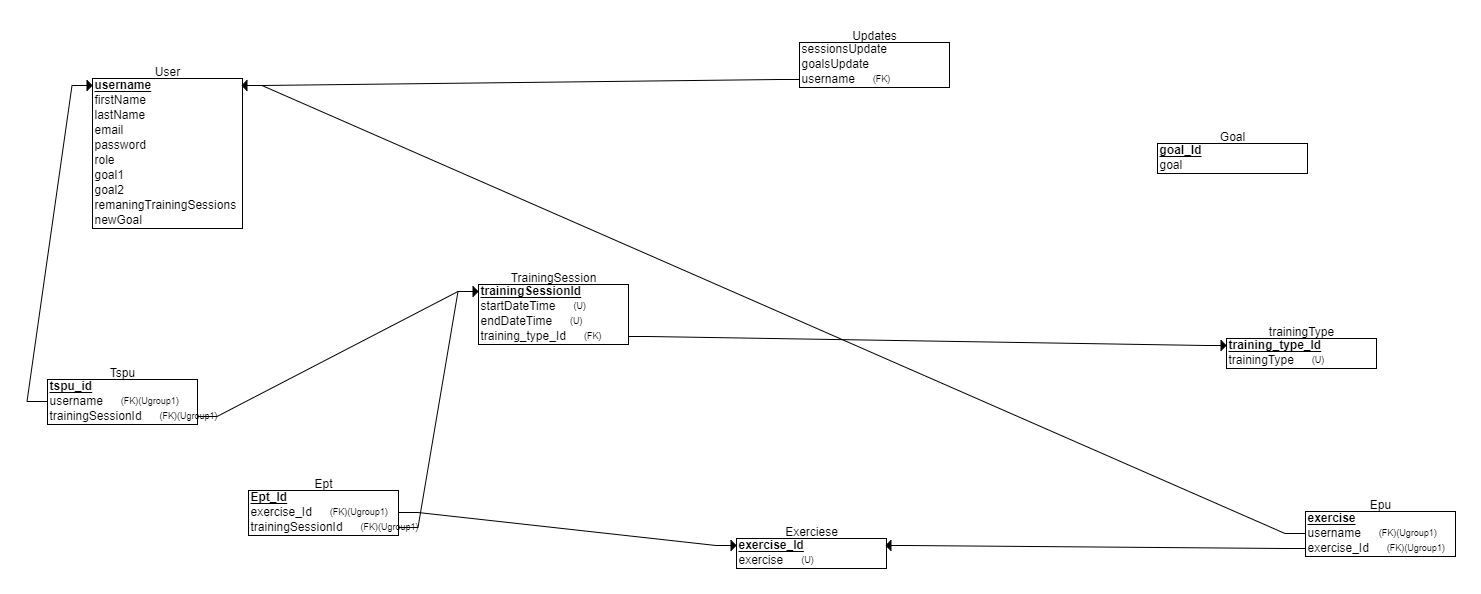
\includegraphics[scale=0.3]{dijagrami/image (8).png} %veličina slike u odnosu na originalnu datoteku i pozicija slike
				\centering
				\caption{dijagram baze podataka}
				\label{fig:diagramRAZ2}
			\end{figure}
			
			
		\section{Dijagram razreda}
		
			{Na sljedećij nekoliko fotografija(4.3, 4.4, 4.5, 4.6 te 4.7) prikazani su razredi backenda koji pripadaju spring arhitektur točnije troslojnom modelu. Konkretno na fotografiji 4.3 prikazani su controller razredi, na fotografiji 4.4 razredi modela, na fotografiji 4.5 razredi repozitorija, na fotografiji 4.6 razredi pripadnih entiteta te na fotografiji 4.7 razredi servisa .}\\
			
			{Nadalje dijagrami su organizirani tako da zrcale  kompontente backend infrastrukture kako bih dijagrami bili pregledniji te logički smisleni.}\\
			
			
			\begin{figure}[H]
				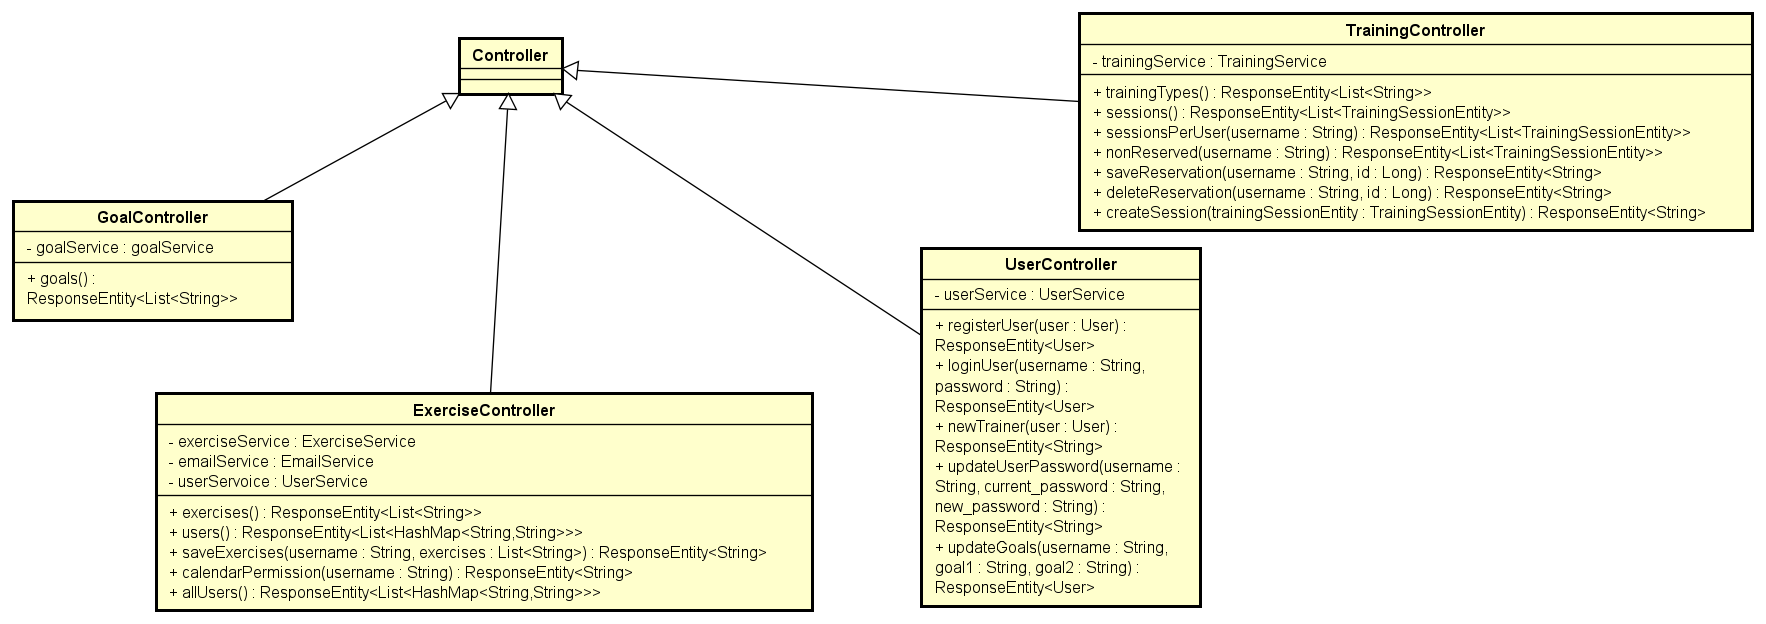
\includegraphics[scale=0.3]{dijagrami/ControllerFinalVersion.png} %veličina slike u odnosu na originalnu datoteku i pozicija slike
				\centering
				\caption{dijagram razreda - Dijagram kontrolera}
				\label{fig:diagramRAZ1}
			\end{figure}
		
			
			
			\begin{figure}[H]
				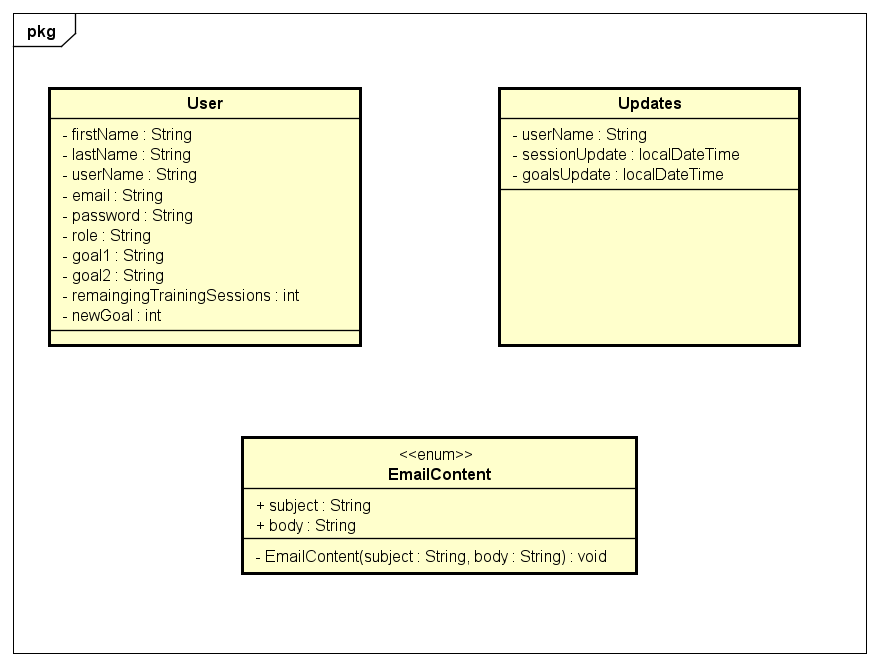
\includegraphics[scale=0.6]{dijagrami/ModelsFinalVersion.png} %veličina slike u odnosu na originalnu datoteku i pozicija slike
				\centering
				\caption{dijagram razreda - Dijagram modela}
				\label{fig:diagramRAZ2}
			\end{figure}
			
			{Na fotografiji 4.4 prikazan je dijagram razreda modela koji preslikavaju entitete i atribute istih na temelju modela baze podataka. }
		
			\begin{figure}[H]
				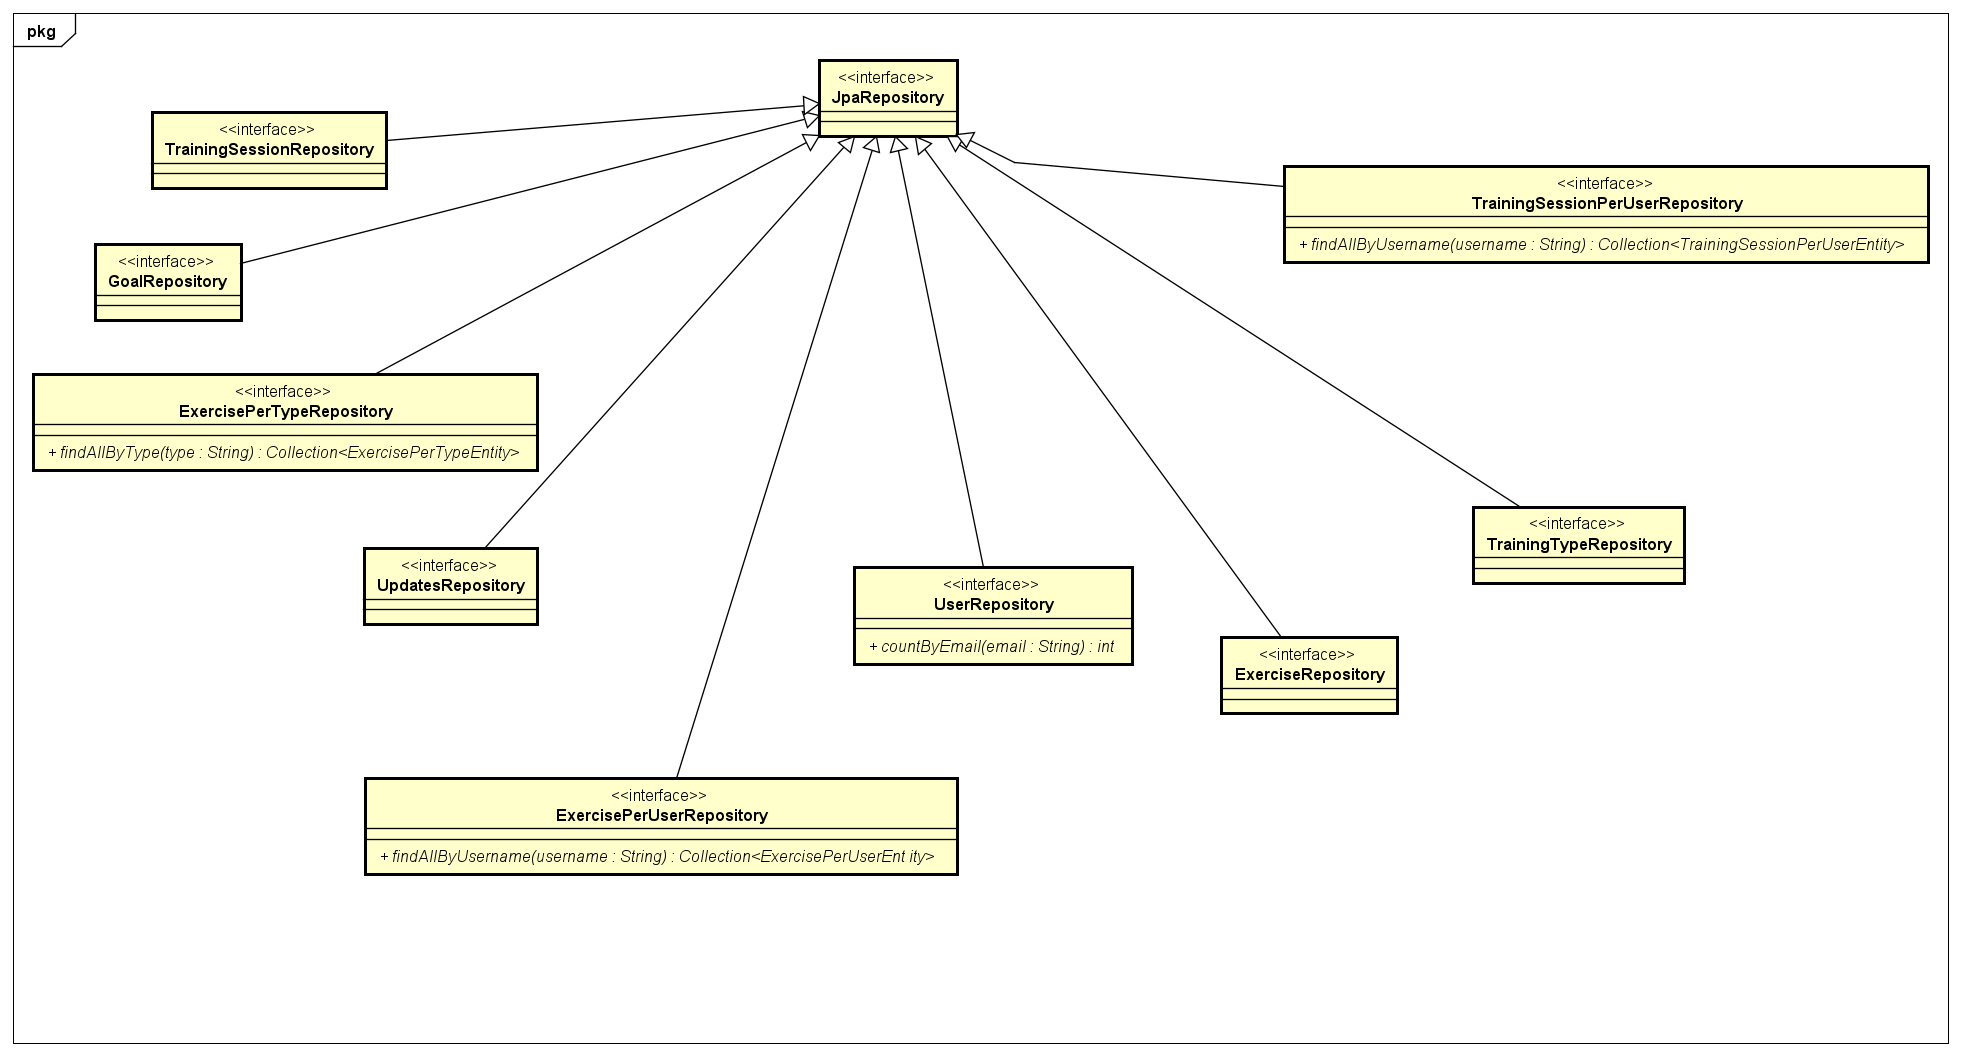
\includegraphics[scale=0.3]{dijagrami/RepositoryFinalVersion.png} %veličina slike u odnosu na originalnu datoteku i pozicija slike
				\centering
				\caption{dijagram razreda - Dijagram repozitorija}
				\label{fig:diagramRAZ3}
			\end{figure}
		
		
			\begin{figure}[H]
				\includegraphics[scale=0.3]{dijagrami/EntitiesFinalVersion.png} %veličina slike u odnosu na originalnu datoteku i pozicija slike
				\centering
				\caption{dijagram razreda - dijagram entiteta}
				\label{fig:diagramRAZ4}
			\end{figure}
		
			\begin{figure}[H]
				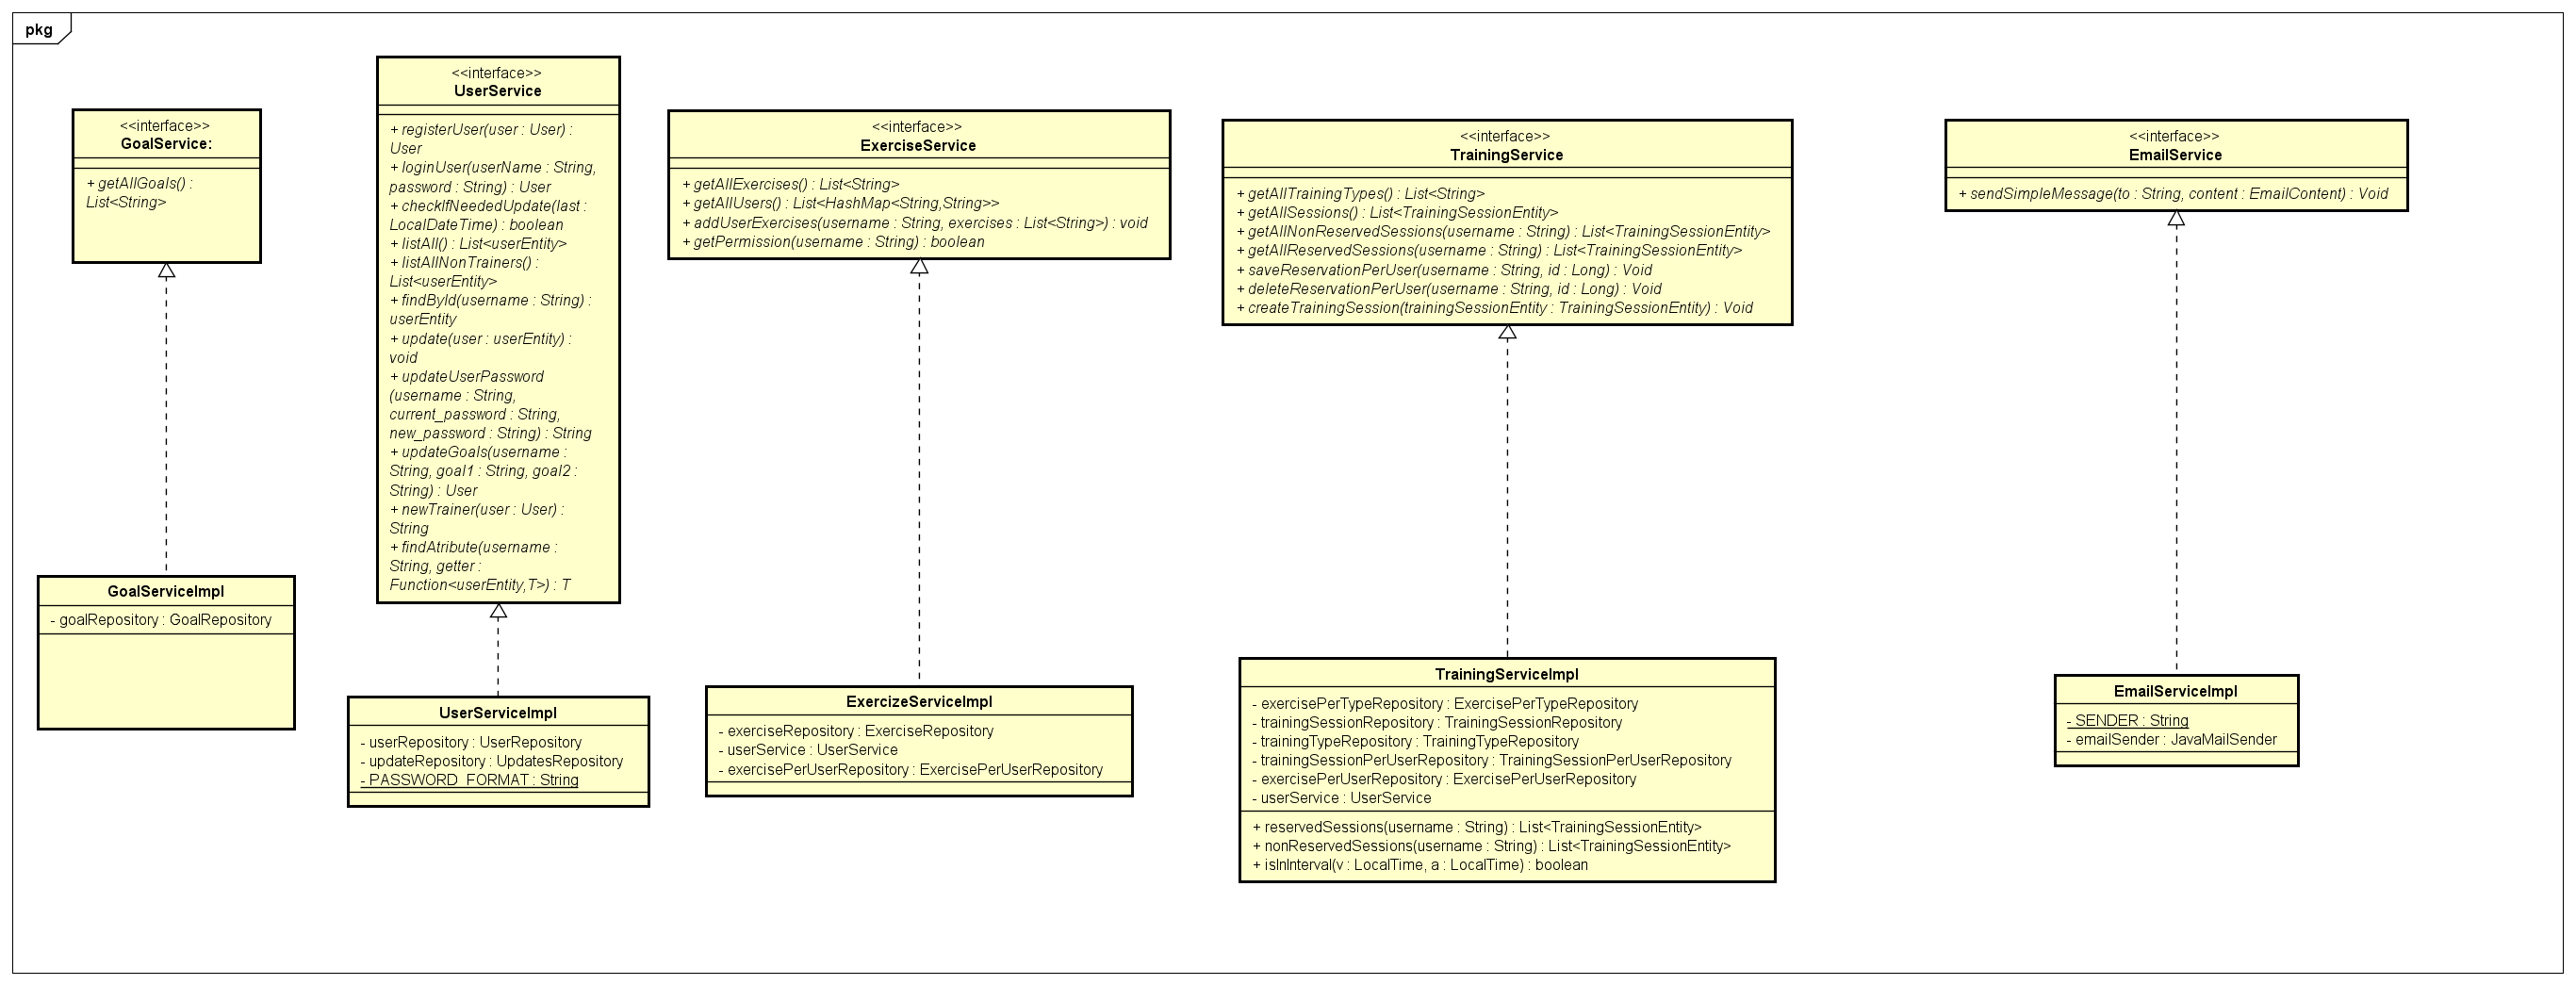
\includegraphics[scale=0.2]{dijagrami/servicesFinalVersion.png} %veličina slike u odnosu na originalnu datoteku i pozicija slike
				\centering
				\caption{dijagram razreda - dijagram servisa}
				\label{fig:diagramRAZ5}
			\end{figure}

		
		
			\textbf{\textit{dio 2. revizije}}\\			
			
			{Prilikom druge predaje projekta dijagram razreda i opisi moraju odgovarati stvarnom stanju implementacije}
			
			
			
			\eject
		
		\section{Dijagram stanja}
			
			{Dijagram stanja opisuje dinamičko ponašanje dijela sustava u vremenu, prikazuje stanja objekta te prijelaze iz jednog stanja u drugo temeljene na događajima. Na slici \ref {fig:dijagramstanja} prikazan je dijagram stanja za registriranog korisnika treninga. Nakon prijave, korisniku se prikazuje njegov personalizirani kalendar. Odabirom određenog termina prikazuju mu se podatci o treningu, to jest od kojih se vježbi sastoji i koliko traje. Ako korisnik ima preostalih sati te određeni termin nije popunjen, korisniku je omogućen gumb "Reserve training session" te klikom na gumb rezervira trening. U slučaju da je korisnikov fond sati nula i/ili da je termin popunjen korisniku je gumb onemogućen te klikom na njega pojavljuje mu se pop-up poruka da ne može rezervirati trening. Također, u zaglavlju stranice korisnik može odabrati neku od ponuđenih mogućnosti. Klikom na "Home page", korisniku se prikazuje naslovna stranica, a klikom na "Profile page" prikazuje mu se stranica s osobni podatcima. Tamo se nalaze osobni podatci korisnika te njegov odabrani cilj. Ukoliko je početak mjeseca, utoliko je korisniku omogućen padajući izbornik za promjenu cilja. Takoeđer, klikom na gumb za uređivanje profila korisniku je omogućena izmjena podataka te mu je prikazan gumb za brisanje korisničkog profila. }
			
			\begin{figure}[H]
				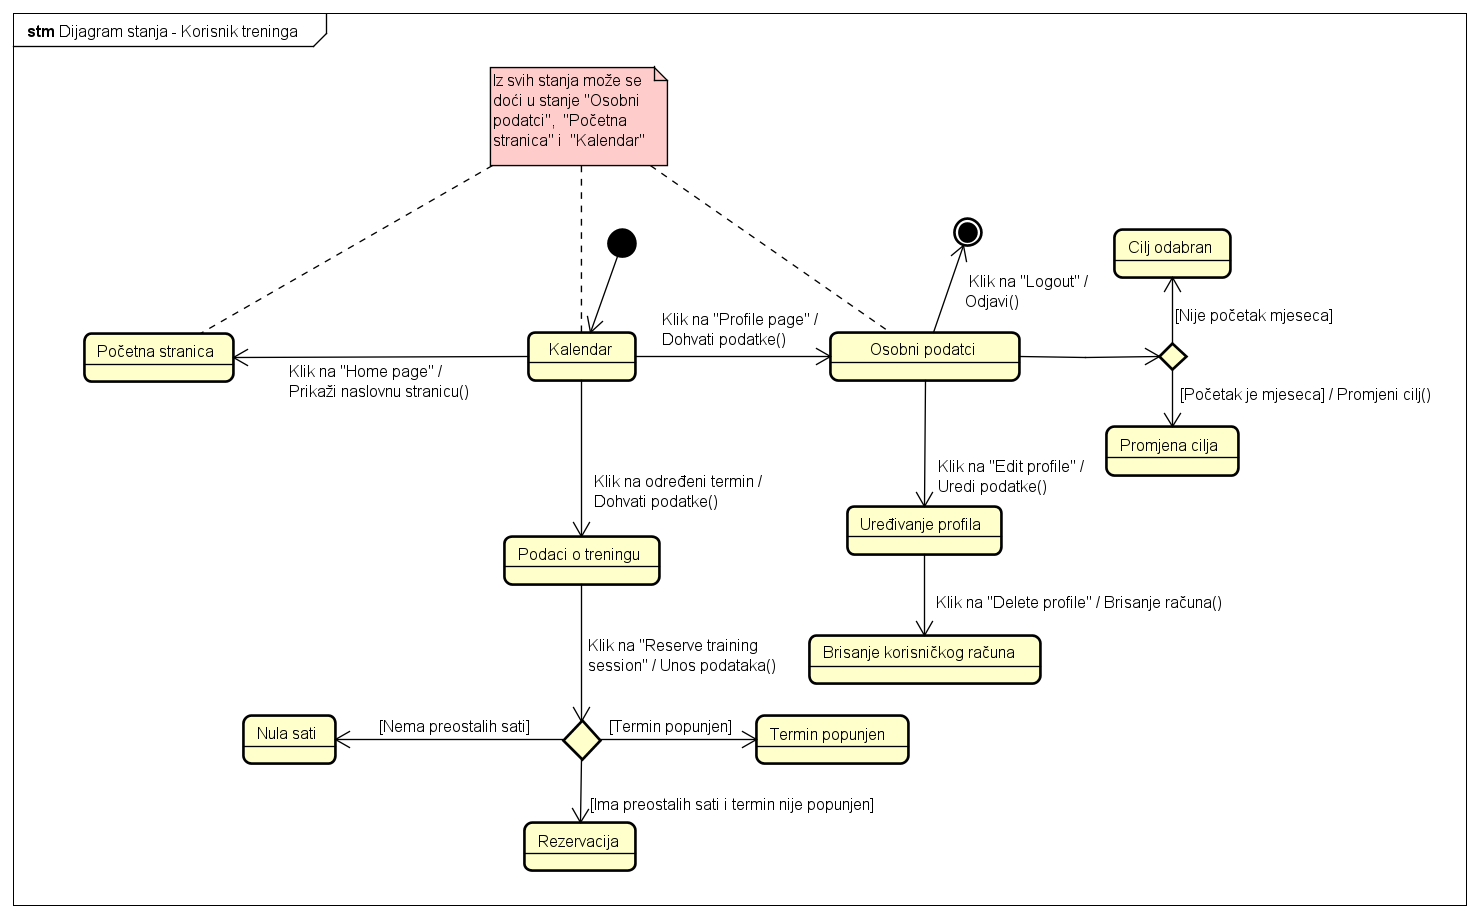
\includegraphics[scale=0.4]{dijagrami/Dijagram stanja - Korisnik treninga.png} %veličina slike u odnosu na originalnu datoteku i pozicija slike
				\centering
				\caption{Dijagram stanja - Korisnik treninga}
				\label{fig:dijagramstanja}
			\end{figure}
			\eject 
		
		\section{Dijagram aktivnosti}
			 
			 {Dijagrami aktivnosti primjenjuju se za modeliranje poslovnih procesa i upravljačkog i podatkovnog toka. Na slici \ref{fig:dijagramaktivnosti} prikazan je proces rezervacije treninga. Korisnik se prijavi u sustav, prikaže mu se personalizirani kalendar i odabire termin treninga za koji želi napraviti rezervaciju. U slučaju da korisnik ima preostaloh sati te da termin nije popunjen, rezervacija se sprema te se prikazuje potvrda rezervacije. Ako je korisnikov fond sati nula ili je termin popunjen, korisniku je onemogućen gumb za rezervaciju te se klikom na njega prikazuje pop-up poruka da ne može rezervirati trening.}
			 
			 \begin{figure}[H]
			 	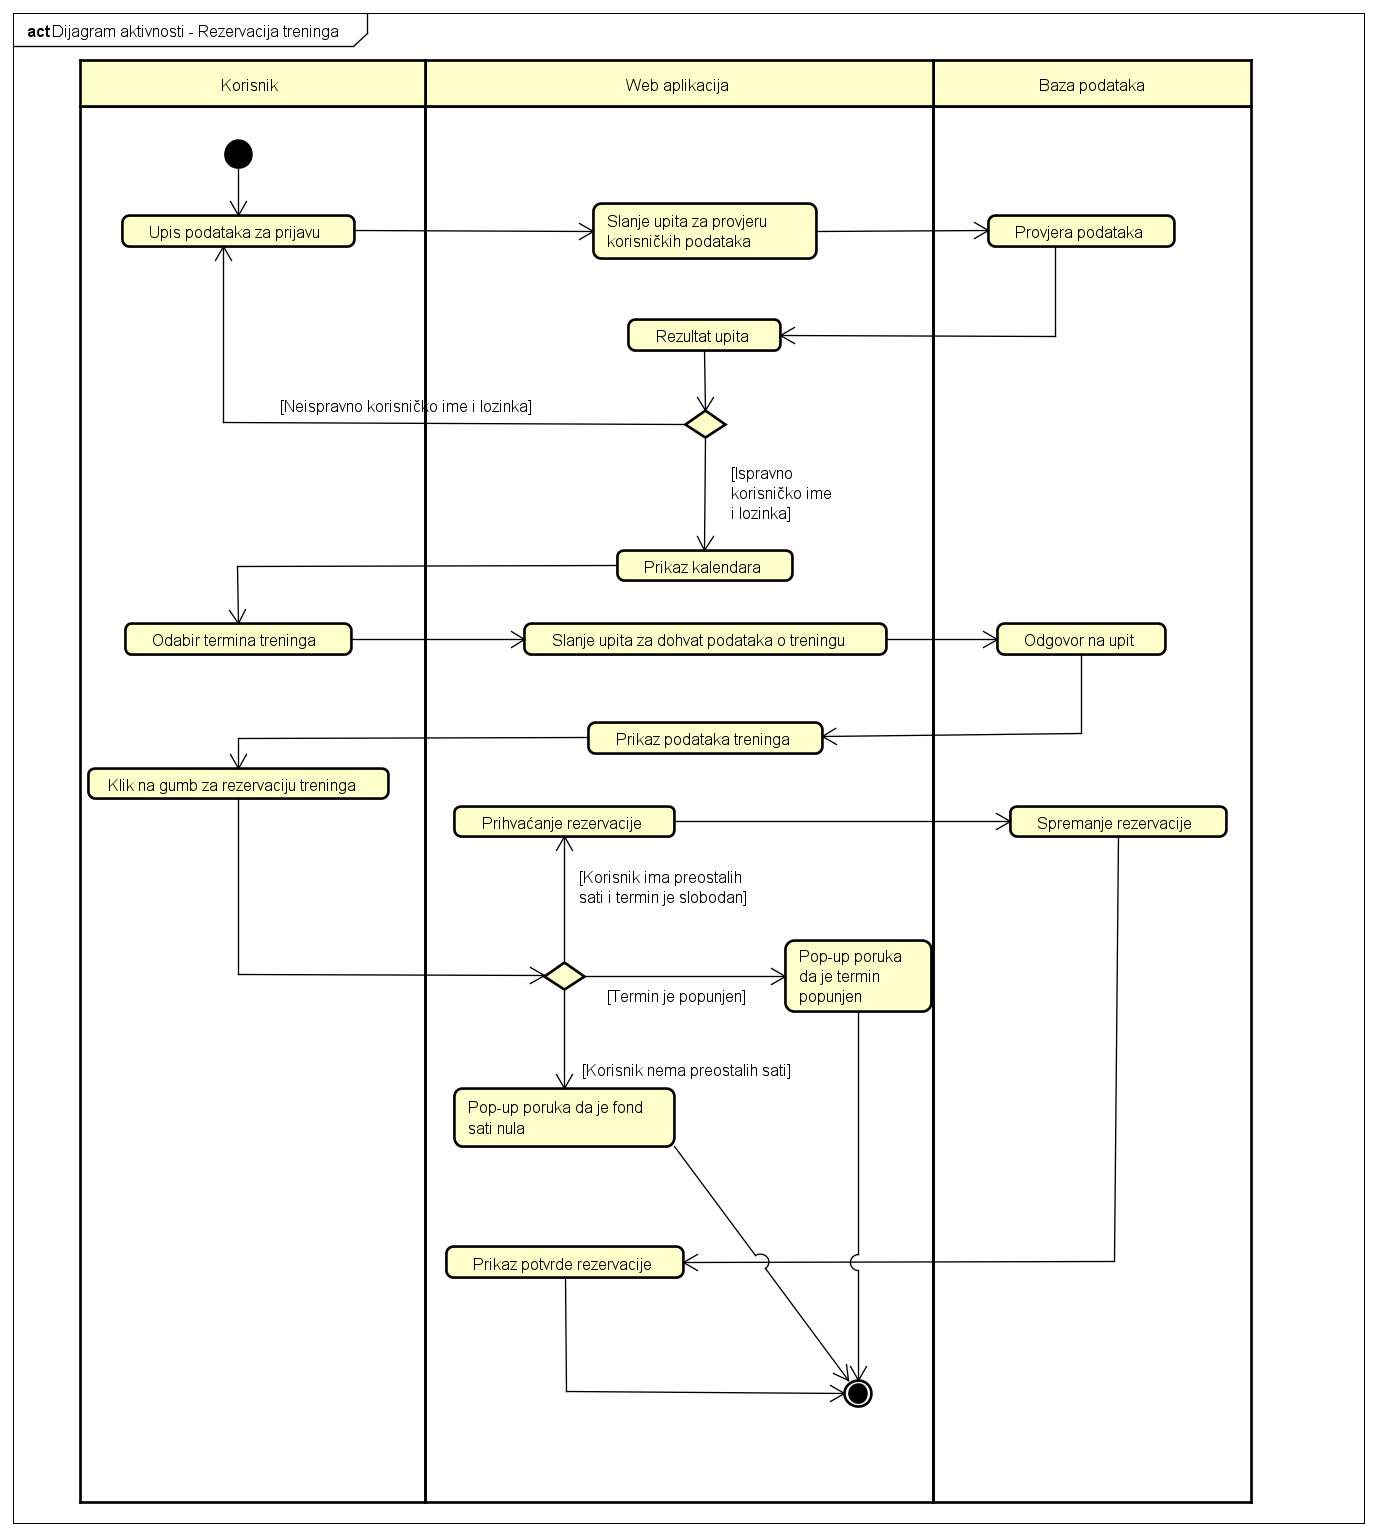
\includegraphics[scale=0.35]{dijagrami/Dijagram aktivnosti - Rezervacija treninga.png} %veličina slike u odnosu na originalnu datoteku i pozicija slike
			 	\centering
			 	\caption{Dijagram aktivnosti - Rezervacija treninga}
			 	\label{fig:dijagramaktivnosti}
			 \end{figure}
			
			\eject
		\section{Dijagram komponenti}
		
		{Dijagram komponenti statički je UML dijagram. Slika \ref {fig:dijagramkomponenti} opisuje organizaciju i međuovisnost
			komponenti, interne strukture i odnose prema okolini. Razlikujemo dva različita sučelja. Preko sučelja za dohvat HTML, CSS i JS datoteka poslužuju se datoteke koje pripadaju klijentskom dijelu aplikacije. App.js komponenta je koja na
			upit s url određuje koja će se datoteka poslužiti na sučelje. Klijentski dio aplikacije se sastoji od niza JavaScript datoteka koje su sakupljene u komponentu Pages. Sve JavaScript datoteke ovise o React biblioteci iz
			koje dohvaćaju gotove komponente kao što su gumbi i forme. Preko sučelja za dohvat JSON podataka pristupa se REST API komponenti. REST API poslužuje podatke koji pripadaju poslužiteljskom dijelu aplikacije. Repository komponenta
			služi za dohvaćanje tablica iz baze podataka pomoću SQL upita. React-view komponenta preko dostupnih sučelja komunicira s aplikacijom te ovisno o akcijama korisnika osvježava prikaz i dohvaća nove podatke.}
		
			\begin{figure}[H]
				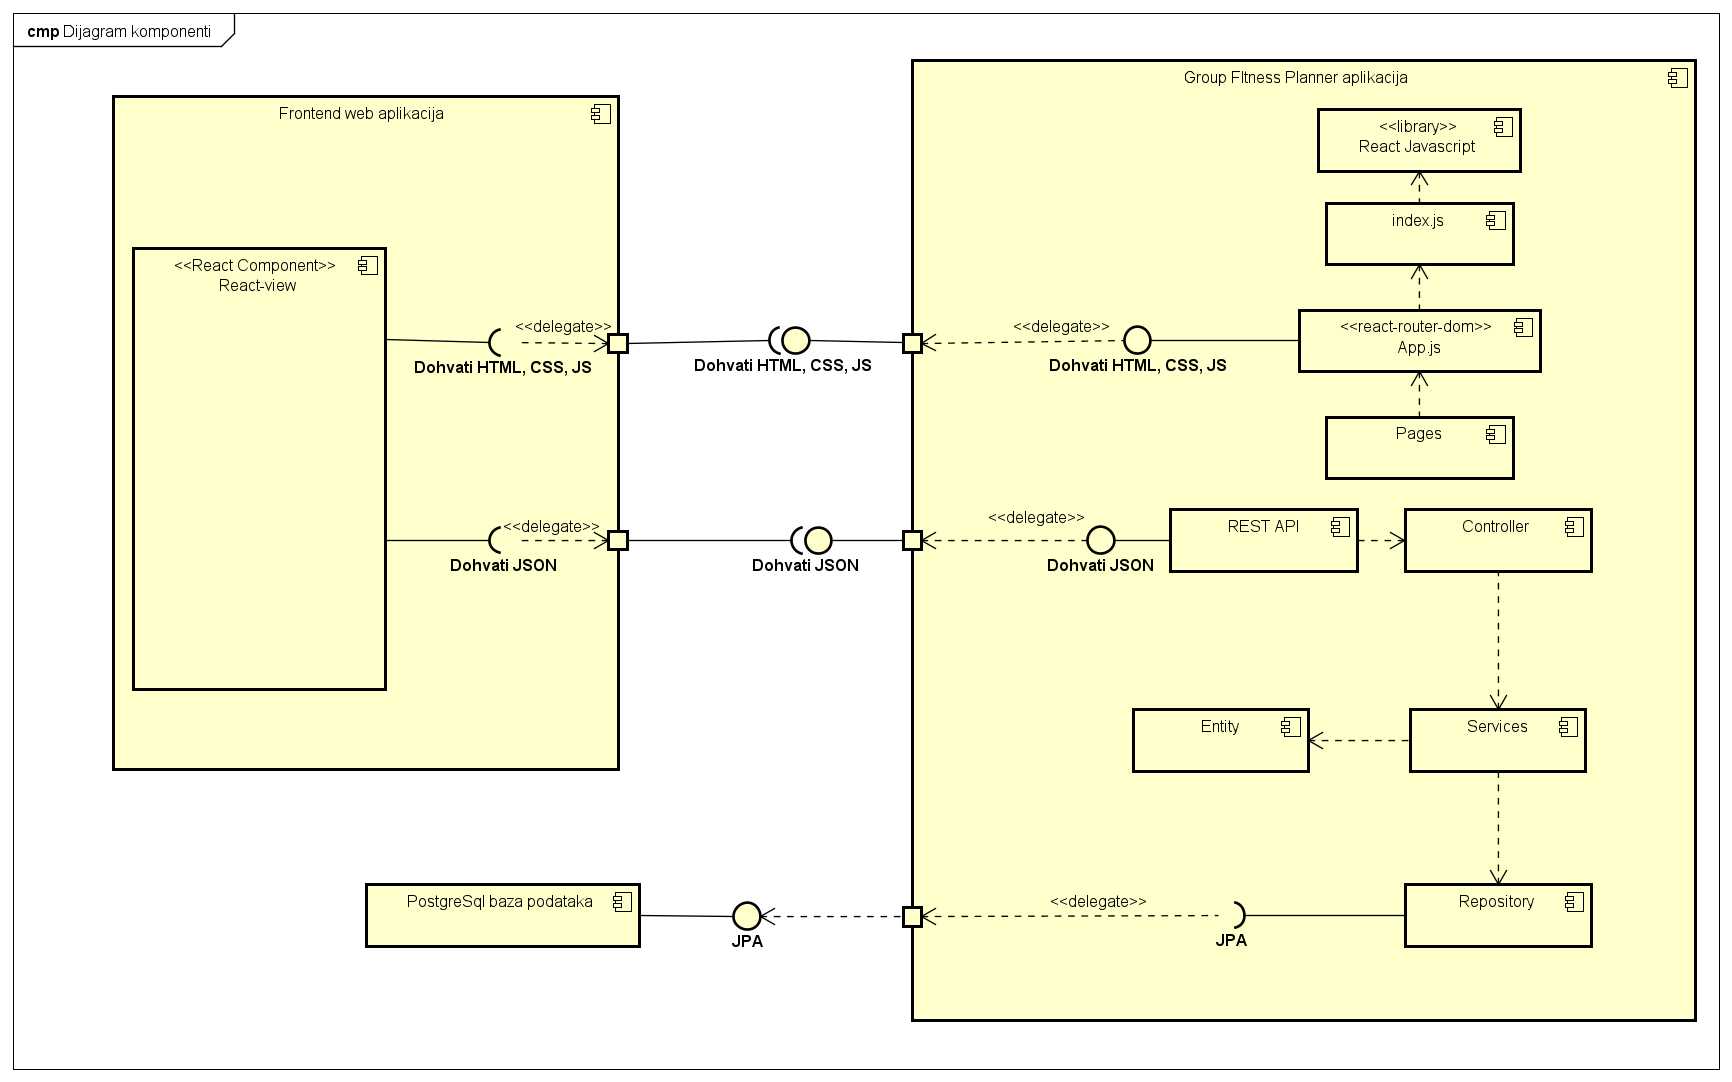
\includegraphics[scale=0.35]{dijagrami/Dijagram komponenti.png} %veličina slike u odnosu na originalnu datoteku i pozicija slike
				\centering
				\caption{Dijagram komponenti}
				\label{fig:dijagramkomponenti}
			\end{figure}

	\chapter{Implementacija i korisničko sučelje}
		
		
		\section{Korištene tehnologije i alati}
		
			
			 {Organizacija te raspodjela i komunikacija tima odvijala se preko aplikacije \underline{WhatsApp\textsuperscript{1}}. Nadalje UML dijagrami su su napravljeni u alatu \underline{Atash Professional\textsuperscript{2}} te je za upravljanje kodom korišten \underline{Git\textsuperscript{3}}, a cijeli projekt je dostupan na udaljenom repozitoriju u sklopu web aplikacije \underline{GitLab\textsuperscript{4}}}.\\
			
			
			{Pri konstrukciji front end-a korišten je \underline{Microsoft Visual studio code\textsuperscript{5}} - uređivač koda  tvrtke Microsoft. Primarno se koristi kao uređivač koda te sadrži podršku za razvojne operacije kao što su debuggiranje, izvođenje zadataka te verzioniranje. Nadalje pri konstrukciji back end-a korišten  je \underline{IntelliJ IDEA\textsuperscript{6}} integrirano radno okruženje (IDE) tvrtke JetBrains. Primarno se koristi za razvoj softvera napisanog u Javi, Kotlinu te drugim jezicima temeljenim na JVM-u(Java virtual machine) }.\\
			
			{Web aplikacija je napisana koristeći radni okvir \underline{Spring boot\textsuperscript{7}} i jezik \underline{Java\textsuperscript{8}} za izradu back end-a te za izradu front end-a korišten je jezik \underline{JavaScript\textsuperscript{9}}  odnosno njegova biblioteka otvorenog tipa  \underline{React\textsuperscript{10}} održavana od strane tvrtke Meta te neovisni programera. React se najčšće  koristi kao osnova u razvoju web aplikacija. Složene aplikacije u Reactu  zahtijevaju korištenje dodatnih biblioteka za interakciju s API-jem. Radni okvir Spring boot je ekstenzija Spring radnog okvira te eliminira konfiguranciju okvirne ploče potrebne za postavljanje spring aplikacije }.\\
			
			{Baza podataka pisana je u \underline{PostgreSql\textsuperscript{11}} SQL jeziku te je za njeno kreiranje korišten radna okolina \underline{PgAdmin\textsuperscript{12}}. Nadalje aplikacija je podignuta na web pomoću oblaka \underline{Render\textsuperscript{13}}  }.
			
			\noindent\rule{8cm}{0.4pt}
			
			\noindent\textsuperscript{1}https://www.whatsapp.com/ \\
			\textsuperscript{2}https://astah.net/products/astah-professional/ \\
			\textsuperscript{3}https://git-scm.com/ \\
			\textsuperscript{4}https://about.gitlab.com/ \\
			\textsuperscript{5}https://code.visualstudio.com/ \\
			\textsuperscript{6}https://www.jetbrains.com/idea/ \\
			\textsuperscript{7}https://spring.io/projects/spring-boot \\
			\textsuperscript{8}https://www.java.com/en/ \\
			\textsuperscript{9}https://www.javascript.com/ \\
			\textsuperscript{10}https://reactjs.org/ \\
			\textsuperscript{11}https://www.postgresql.org/ \\
			\textsuperscript{12}https://www.pgadmin.org/ \\
			\textsuperscript{13}https://render.com/ \\
			
			
			
			
			\eject 
		
	
		\section{Ispitivanje programskog rješenja}
			
		
	
			
			\subsection{Ispitivanje komponenti}
		
			
			\textbf{Ispitni slučaj 1: Uspješno stvaranje trenera}\\
				\begin{verbatim}
					@Test
					public void testCreatingNewTrainerSuccessfully() throws Exception{
					
						User mockUser = UserGeneratingUtil.createMockUser();
						
						when(userService.newTrainer(mockUser)).thenReturn("success")
						
						mvc.perform(post("/new-trainer").contentType(MediaType.APPLICATION_JSON).content(objectMapper.writeValueAsString(mockUser))).
							andExpect(status().isOk())
							.andExpect(content().string(("success")));
							
				}
				\end{verbatim}\\\\
			
				\textbf{Ispitni slučaj 2: Neuspješno stvaranje trenera}\\\\
				
				\begin{verbatim}
					@Test
					public void testCreatingNewTrainerSuccessfully() throws Exception{
								
									User mockUser = UserGeneratingUtil.createMockUser();
									
									when(userService.newTrainer(mockUser)).thenThrow(new REquest DeniedException("Username: " + mockUser.getUsername() + " is already taken."));
									
									mvc.perform(post("/new-trainer").contentType(MediaType.APPLICATION_JSON).content(objectMapper.writeValueAsBytes(mockUser))).
											andExpect(status().is4xxClientError());
											
											
					}
				\end{verbatim}\\
		
				\begin{figure}[H]
				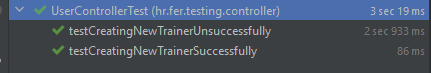
\includegraphics[scale=1]{dijagrami/2.png} %veličina slike u odnosu na originalnu datoteku i pozicija slike
				\centering
				\caption{Rezultati ispitnih slučajeva 1 i 2}
				\label{fig:ispitnislucaj12rez}
			\end{figure}\\\\
		
			
			\textbf{Ispitni slučaj 3: dohvaćanje treninga }\\
			
			\begin{verbatim}
				@Test
				public void testGetAllSessions() {
						
						TrainingSessionEntity mockTs = TrainingGeneratingUtil.createMockSession();
						
						when(trainingSessionRepository.findAll()).thenReturn(List.of(mockTs));
						
						verify(trainingSessionRepository, times(1)).findAll();
						
						Assert.assertEquals(found.size(), 1);
						
				}
			\end{verbatim}\\
			
			
				\begin{figure}[H]
				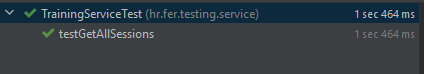
\includegraphics[scale=1]{dijagrami/4.png} %veličina slike u odnosu na originalnu datoteku i pozicija slike
				\centering
				\caption{Rezultat ispitnog slučaja 3}
				\label{fig:ispitnislucaj3rez}
			\end{figure}\\\\
		
		
			\textbf{Ispitni slučaj 4: Prikaz svih ne trenera}\\\\
		
			\begin{verbatim}
				
				@Test
				public void testListingAllNonTrainers() {
					
					User mockUser = UserGeneratingUtil.createMockUser();
					
					UserEntity mockUserEntity = USerEntity.from(mockUser);
					
					when(userRepository.findAll()).thenReturn(List.of(mockUserEntity));
					
					List<UserEntity> found = userService.listAllNonTrainers();
					
					verify(userRepository, times(1)).fidnAll();
					
					Assert.assertEquals(found.size(), 0)
					
			}
			\end{verbatim}\\\\
		
			\textbf{Ispitni slučaj 5: Neuspješno dodavanje novog trenera}\\
			
			\begin{verbatim}
					@Test
					public void testAddingNewTrainerUnsuccessfully() {
						
						User mockUser = UserGeneratingUtil.createMockUser();
						
						UserEntity mockUserEntity = USerEntity.from(mockUser);
						
						when(userRepositroy.findById(mockUser.getUsername())).thenReturn(Optional.of(mockUserEntity));
						
						when(userRepositroy.countByEmail(mockUser.getEmail())).thenReturn(0);
						
						assertThrows(requestDeniedException.class, () -> userService.newTrainer(mockUser));
						
						verfy(userRepository, times(1)).findById(mockUser.getUsername());
						
						verfy(userRepository, times(1)).countByEmail(mockUser.getEmail());
						
					}
			\end{verbatim}\\\\
		
			\textbf{Ispitni slučaj 6: Neuspješno pronalaženja korisnika po ID-u}\\
		
			\begin{verbatim}
				@Test
				public void testFindingUSerByIdUnsuccessfully() {
						
						User mockUser = UserGeneratingUtil.createMockUser();
						
						UserEntity mockUserEntity = USerEntity.from(mockUser);
						
						String mockUsername= "stella";
						
						when(userRepository.findById(mockUsername)).thenReturn(Optional.empty());
						
						UserEntity found = userService.findById(mockUsername);
						
						verfiy(userRepository, times(1)).findById(mockUsername);
						
						Assert.assertEquals(found, null);
							
			}
			\end{verbatim}\\
		
				\begin{figure}[H]
				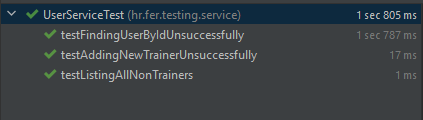
\includegraphics[scale=1]{dijagrami/6.png} %veličina slike u odnosu na originalnu datoteku i pozicija slike
				\centering
				\caption{Rezultati ispitnih slučajeva 4, 5 i 6}
				\label{fig:ispitnislucaj3rez}
			\end{figure}\\\\
			
			\subsection{Ispitivanje sustava}
				
				\textbf{Ispitni slučaj 1: Uspješan pristup kalendaru}
				
				\textbf{Ulaz:}
				\begin{enumerate}
					\item Otvaranje početne stranice web aplikacije
					\item pritisak na gumb "login"
					\item unošenje podataka (korisnik posjeduje postojeći račun)
					\item redirect na stranicu kalendara
				\end{enumerate}
				\textbf{Izlaz:}
				\begin{enumerate}
					\item prikazuje se početna stranica
					\item gumb nas vodi na stranicu login
					\item uspješna prijava
					\item prikaz stranice kalendara
				\end{enumerate}
				\textbf{Rezultati:} {Aplikacija je uspješno izvela sve korake testa. \color{green} Aplikacija je prošla test.}\\\\
				
				
					\begin{figure}[H]
					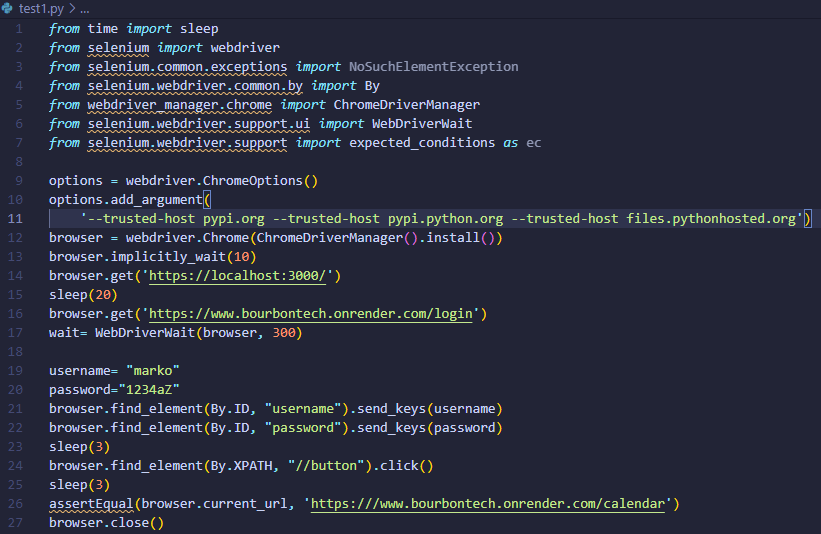
\includegraphics[scale=0.4]{dijagrami/test1.png} %veličina slike u odnosu na originalnu datoteku i pozicija slike
					\centering
					\caption{Izvorni kod ispitnog slučaja 1}
					\label{fig:ispitnislucaj1}
				\end{figure}\\
				
				
					\textbf{Ispitni slučaj 2: Neuspješan pristup kalendaru}
				
				\textbf{Ulaz:}
				\begin{enumerate}
					\item Otvaranje početne stranice web aplikacije
					\item pritisak na gumb "login"
					\item unošenje podataka (korisnik ne posjeduje postojeći račun)
					\item redirect na stranicu neuspjele prijave 
				\end{enumerate}
				\textbf{Izlaz:}
				\begin{enumerate}
					\item prikazuje se početna stranica
					\item gumb nas vodi na stranicu login
					\item uneseni podaci ne odgovaraju ni jednom postojećem računu
					\item prikaz stranice neuspjele prijave
				\end{enumerate}
				\textbf{Rezultati:} {Sve komponente testa su uspješno zadovoljene od strane aplikacije. \color{green} Aplikacija je prošla test.}\\\\
			
					\begin{figure}[H]
					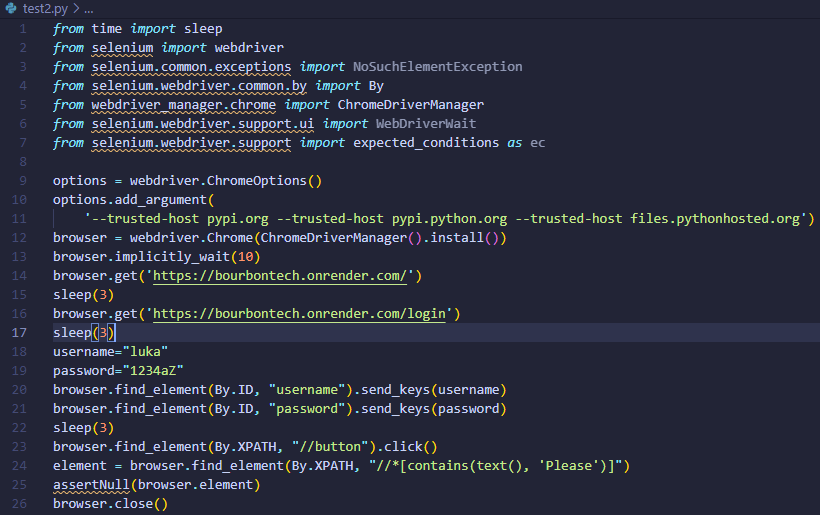
\includegraphics[scale=0.4]{dijagrami/test2.png} %veličina slike u odnosu na originalnu datoteku i pozicija slike
					\centering
					\caption{Izvorni kod ispitnog slučaja 2}
					\label{fig:ispitnislucaj2}
				\end{figure}\\
				
					\textbf{Ispitni slučaj 3: Promjena lozinke}
				
				\textbf{Ulaz:}
				\begin{enumerate}
					\item Otvaranje početne stranice web aplikacije
					\item pritisak na gumb "login"
					\item unošenje podataka (korisnik posjeduje postojeći račun)
					\item redirect na stranicu kalendara
					\item otvaranje stranice profila
					\item pritisak na gumb "change password"
					\item unos stare pa zatim nove lozinke
					\item pritisak na gumb "save"
					\item pritisak na gumb "logout"
					\item pritisak na gumb "login"
					\item prijava s promjenjenim podacima
					\item redirect na stranicu kalendara
				\end{enumerate}
				\textbf{Izlaz:}
				\begin{enumerate}
					\item prikazuje se početna stranica
					\item gumb nas vodi na stranicu login
					\item uspješna prijava
					\item prikaz stranice kalendara
					\item prikaz stranice profila
					\item prikaz forme za promjenu lozinke
					\item nova lozinka spremljena
					\item korisnik odjavljen
					\item gumb nas vodi na stranicu login
					\item uspješna prijava
					\item prikaz stranice kalendara
				\end{enumerate}
				\textbf{Rezultati:} {Aplikacija je pravilno i efikasno izvela zahtjeve testa. \color{green} Aplikacija je prošla test.}\\\\
				
					\begin{figure}[H]
					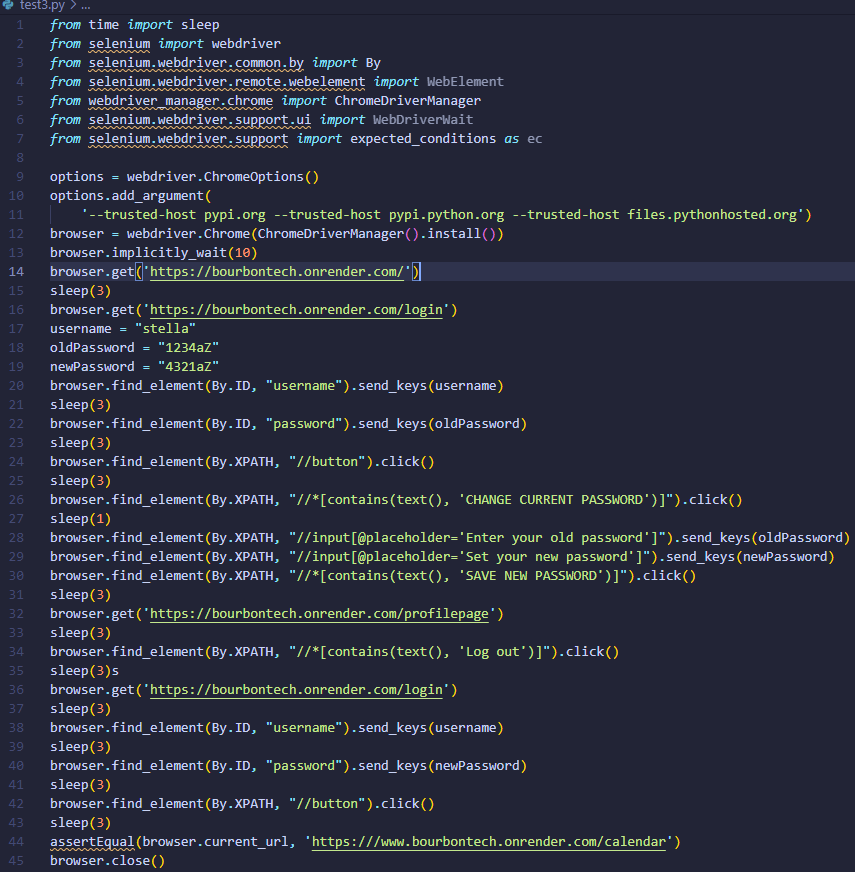
\includegraphics[scale=0.4]{dijagrami/test3.png} %veličina slike u odnosu na originalnu datoteku i pozicija slike
					\centering
					\caption{Izvorni kod ispitnog slučaja 3}
					\label{fig:ispitnislucaj3}
				\end{figure}\\
				
				
				\textbf{Ispitni slučaj 4: Rezervacija treninga}
				
				\textbf{Ulaz:}
				\begin{enumerate}
					\item Otvaranje početne stranice web aplikacije
					\item pritisak na gumb "login"
					\item unošenje podataka (korisnik posjeduje postojeći račun)
					\item redirect na stranicu kalendara
					\item klik na gumb "reservation"
					
				\end{enumerate}
				\textbf{Izlaz:}
				\begin{enumerate}
					\item prikazuje se početna stranica
					\item gumb nas vodi na stranicu login
					\item uspješna prijava
					\item prikaz stranice kalendara
					\item smanjivanje fonda sati za jedan
				\end{enumerate}
				\textbf{Rezultati:} {Testiranje aplikacije je završilo uspješno. \color{green} Aplikacija je prošla test.}\\\\
				
				
					\begin{figure}[H]
					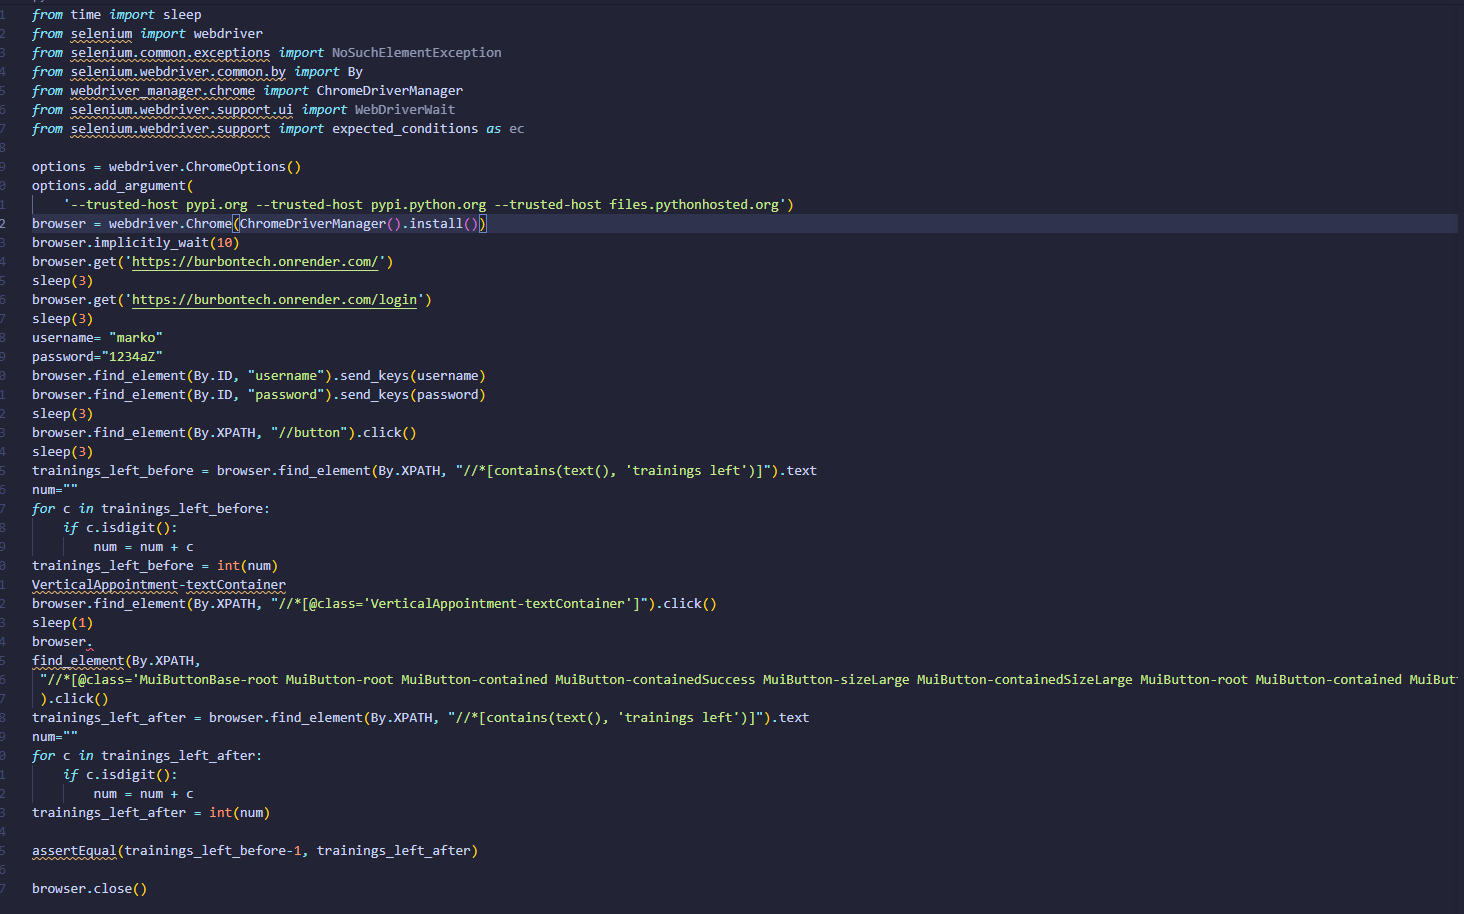
\includegraphics[scale=0.4]{dijagrami/test4.png} %veličina slike u odnosu na originalnu datoteku i pozicija slike
					\centering
					\caption{Izvorni kod ispitnog slučaja 4}
					\label{fig:ispitnislucaj4}
				\end{figure}\\
		
		\section{Dijagram razmještaja}
			
			{Dijagrami razmještaja su strukturni statički UML dijagrami koji opisuju topologiju sustava i usredotočeni su na odnos sklopovskih i programskih dijelova. Na strani poslužitelja se nalazi web poslužitelj te poslužitelj baze podataka. Dok se na strani klijenta nalazi web preglednik kojim korisnik pristupa aplikaciji. Sustav je koncipiran na arhitekturi "klijent-poslužitelj" te se komunikacija odvija putem HTTP veze}. \\
			
			
			\begin{figure}[H]
				\includegraphics[scale=0.4]{dijagrami/dijagramRazmještaja.png} %veličina slike u odnosu na originalnu datoteku i pozicija slike
				\centering
				\caption{dijagram razmještaja }
				\label{fig:diagramrazmještaja}
			\end{figure}
			
			\eject 
		
		\section{Upute za puštanje u pogon}
		
			
			
			\textbf{Priprema backend-a za deploy na Render}\\
		
			{Po potrebi dodati env. varijable u run konfiguraciju vašeg IDE-a. Zatim dodati Dockerfile uz napomenu da u direktoriju docker postoje dvije verzije, za Maven i Gradel. Nadalje ukoliko se mijenja lokacija DockerFile-a pripaziti na putanju unutra "COPY" naredbi u DockerFile skripti. U application.properties postaviti property server.servlet.context-path na /api kao prefiks svim zahtjevima na backend. }.\\
			
			\noindent\textbf{Priprema frontend-a za deploy na Render}\\
			
			{U package.json potrebno je dodati dependency-e neophodne za deploy to jest primarno http-proxy-middleware, dontev te express. Zatim potrebno je dodati /src/setupProxy.js koji služi kao proxy server za lokalni development (preusmjerava api pozive na localhost:8080) odnosno kada se koristi "react-scripts start" skripta. Nadalje potrebno je dodati app.js u kojem se nalazi express server za produkcijski proxy te poosluživanje frontend-a. Također potrebno je u package.json izmjeniti \begin{verbatim}
					"build": "yarn install && react-scripts build"\end{verbatim}  te dodati \begin{verbatim}
					"start-prod": "node app.js"
				\end{verbatim} }.\\
			
			\noindent\textbf{Deploy}\\
			
			\textbf{Kreiranje baze podataka}\\
				{Potrebno je u Render dashboard-u izvesti sljedeće komande :
				\begin{itemize}
					\item New $\Rightarrow$ PostgreSQL
					\item Postaviti ime baze i opcionalno username za korisnika baze (password je automatski generiran)
					\item Region Frankfurt
					\item Create Database
					\item Free plan baza podataka ima max pohranu od 1GB 
			\end{itemize}}.\\
			\textbf{Kreiranje backend-a}\\
				{Potrebno je u Render dasboard-u izvesti sljedeće komande :
					\begin{itemize}
						\item New $\Rightarrow$ Web Service
						\item Povezati Gitlab racun, nakon čega su za odaabir dostupni svi projekti na koje imate prava pristupa
						\item Stisnuti connect pored odgovarajućeg projekta
						\item Postaviti ime za servis(postaje dio web adrese)
						\item Rot directory postaviti na progi-be
						\item Environment Docker
						\item Region Frankfurt
						\item Na dnu proširiti advanced
						\item Dodati potrebne environment varijable te kopirati vrijednosti iz postavki baze podataka na Renderu. 
						\item Ako je dodan Spring Boot Actuator postaviti /api/actuator/health kao Healt Check Path
						\item Postaviti putanju za DOckerfile ovisno o pacage menageru 
						\item Stisnuti Create Web Service
				\end{itemize}}
			\textbf{Kreiranje frontend-a}\\
				{Potrebno je u Render dashboard-u izvesti sljedeće komande :
					\begin{itemize}
						\item New $\Rightarrow$ Web Service
						\item  Povezati Gitlab racun, nakon čega su za odaabir dostupni svi projekti na koje imate prava pristupa
						\item Stisnuti connect pored odgovarajućeg projekta
						\item Postaviti ime za servis(postaje dio web adrese)
						\item Rot directory postaviti na progi-fe
						\item Environment Node
						\item Region Frankfurt
						\item Build command postaviti na yarn build, a Start Command yarn start-prod
						\item Na dnu proširiti advanced
						\item Dodati potrebne environment varijable -API\_BASE\_URL postaviti na adresu deployanog backend-a aplikacije dostupne na Render dashboardu
						\item Stisnuti Create Web Service
				\end{itemize}}.\\
			
			
			\eject 
	\chapter{Zaključak i budući rad}
		 
		 {Naš projektni zadatak bio je razvoj web aplikacije za rezervaciju treninga uz dodatak personalizirane ponude treninga ovisno o odabranim ciljevima korisnika. Provedba projekta bila je podijeljena u dvije faze. }
		 
		 {Prva faza projekta odvijala se u prvom ciklusu semestra. Glavni fokus bio je na okupljanju tima, raspodjeli poslova te dokumentaciji projekta. Prva revizija dokumentacija temeljila se na opisu projektnog zadatka, obrascima uporabe, dijagramima obrazaca uporabe, sekvencijskim dijagramima i dijagramima razreda. Definiranje funkcionalnih zahtjeva uvelike je olakšalo daljnji rad na aplikaciji. Također, izrada vizualnih prikaza idejnih rješenja aplikacije pomogla je svim članovima tima kod implementacije. }
		 
		 {Druga faza projekta odvijala se u drugom ciklusu semestra te je glavni fokus bio na programskom dijelu aplikacije. U odnosu na prvu fazu, članovi tima puno su više radili samostalno te su ssastanci bili puno rjeđi. Osim realizacije same aplikacije, u drugoj fazi potrebno je bilo dokumentirati ostatak UML dijagrama i provesti ispitivanje programskog rješenja. }
		 
		 {Jedina funkcionalnost koju nismo implementirali u potpunosti je ta da treneri unose pravila koje se odnose na rezervaciju termina svih korisnika. Naime, odlučili smo kako nam je puno jednostavnije da su ta pravila već određena u aplikaciji, a ne da ih trener sam unosi.}
		 
		 {Sudjelovanje na ovom projektu svim članovima tima bilo je jako korisno iskustvo. Imali smo priliku raditi u timu te smo na taj način naučili surađivati s drugim članovima i zajednički dolaziti do optimalnih rješenja. Zaključili smo da je najvažnija dobra komunikacija među članovima. Komunikacija među članovima tima uglavnom se odvijala preko Whatsappa te su tako svi članovi tima bili informirani o napretku projekta. Smatramo da smo vrlo dobro odradili zadatak, iako postoji prostora za napredak. }
		
		\eject 
	\chapter*{Popis literature}
		\addcontentsline{toc}{chapter}{Popis literature}
	
		\textit{Popisati sve reference i literaturu koja je pomogla pri ostvarivanju projekta.}
		
		
		\begin{enumerate}
			
			
			\item  Programsko inženjerstvo, FER ZEMRIS, \url{http://www.fer.hr/predmet/proinz}
			
			\item  Baze podataka, FER
			\url {https://www.fer.unizg.hr/predmet/bazpod_c}
			
			\item Procesi programskog inženjerstva, FER
			\url {https://www.fer.unizg.hr/_download/repository/Procesi_programskog_inzenjerstva_3_izdanje[1].pdf}
		\end{enumerate}
		
		 
	
	
	\begingroup
	\renewcommand*\listfigurename{Indeks slika i dijagrama}
	%\renewcommand*\listtablename{Indeks tablica}
	%\let\clearpage\relax
	\listoffigures
	%\vspace{10mm}
	%\listoftables
	\endgroup
	\addcontentsline{toc}{chapter}{Indeks slika i dijagrama}


	
	\eject 
		
	\chapter*{Dodatak: Prikaz aktivnosti grupe}
		\addcontentsline{toc}{chapter}{Dodatak: Prikaz aktivnosti grupe}
		
		\section*{Dnevnik sastajanja}
		
		\begin{packed_enum}
			\item  sastanak
			
			\item[] \begin{packed_item}
				\item Datum: 20.10.2022.
				\item Prisustvovali: Luka Vukelić, Stella Balić, Jelena Kulišić, Matko Nikolić, Barbara Pašalić, Tin Pavletić, Jure Rajčić
				\item Teme sastanka:
				\begin{packed_item}
					\item  sastanak s asistentom i demonstratorom
					\item  upoznavanje s temom projekta
				\end{packed_item}
			\end{packed_item}
			
			\item  sastanak
			\item[] \begin{packed_item}
				\item Datum: 26.10.2022.
				\item Prisustvovali: Luka Vukelić, Stella Balić, Jelena Kulišić, Matko Nikolić, Barbara Pašalić, Tin Pavletić, Jure Rajčić
				\item Teme sastanka:
				\begin{packed_item}
					\item  raspodjela poslova po članovima tema
					\item  detaljna razrada teme
				\end{packed_item}
			\end{packed_item}
		 
		 \item  sastanak
		 \item[] \begin{packed_item}
		 	\item Datum: 5.11.2022.
		 	\item Prisustvovali: Luka Vukelić, Stella Balić, Jelena Kulišić, Matko Nikolić, Barbara Pašalić, Tin Pavletić, Jure Rajčić
		 	\item Teme sastanka:
		 	\begin{packed_item}
		 		\item  komentari dosadašnjeg rada
		 		\item  daljnja podjela rada
		 	\end{packed_item}
		 \end{packed_item}
	 
	   \item  sastanak
	   \item[] \begin{packed_item}
	   	\item Datum: 10.11.2022.
	   	\item Prisustvovali: Luka Vukelić, Stella Balić, Jelena Kulišić, Matko Nikolić, Barbara Pašalić, Tin Pavletić, Jure Rajčić
	   	\item Teme sastanka:
	   	\begin{packed_item}
	   		\item  dogovor za popravak dokumentacije
	   		\item  dizajn stranice, komunikacija backenda i frontenda, baza podataka
	   	\end{packed_item}
	   \end{packed_item}
			
			%
			
		\end{packed_enum}
		
		\eject
		\section*{Tablica aktivnosti}

			\begin{longtblr}[
					label=none,
				]{
					vlines,hlines,
					width = \textwidth,
					colspec={X[7, l]X[1, c]X[1, c]X[1, c]X[1, c]X[1, c]X[1, c]X[1, c]}, 
					vline{1} = {1}{text=\clap{}},
					hline{1} = {1}{text=\clap{}},
					rowhead = 1,
				} 
				\multicolumn{1}{c|}{} & \multicolumn{1}{c|}{\rotatebox{90}{\textbf{Luka Vukelić}}} & \multicolumn{1}{c|}{\rotatebox{90}{\textbf{Stella Balić }}} &	\multicolumn{1}{c|}{\rotatebox{90}{\textbf{Jelena Kulišić }}} & \multicolumn{1}{c|}{\rotatebox{90}{\textbf{Matko Nikolić}}} &	\multicolumn{1}{c|}{\rotatebox{90}{\textbf{Barbara Pašalić }}} & \multicolumn{1}{c|}{\rotatebox{90}{\textbf{Tin Pavletić }}} &	\multicolumn{1}{c|}{\rotatebox{90}{\textbf{Jure Rajčić }}} \\  
				Upravljanje projektom 		& 5  &  &  &  &  &  & \\ 
				Opis projektnog zadatka 	&  &  & 7 &  &  &  & \\ 
				
				Funkcionalni zahtjevi       & 5 &  &  &  &  &  &  \\ 
				Opis pojedinih obrazaca 	& 5 &  &  &  &  &  &  \\ 
				Dijagram obrazaca 			& 3 &  &  &  &  & 3 &  \\ 
				Sekvencijski dijagrami 		& 3 &  &  &  &  & 5 &  \\ 
				Opis ostalih zahtjeva 		&  &  & 1  &  &  &  &  \\ 

				Arhitektura i dizajn sustava	 &  &  & 4 &  & &  &  \\ 
				Baza podataka				&  & 3 & 3 &  &  & 3 &   \\ 
				Dijagram razreda 			&  &  &  &  &  & 7 &   \\ 
				Dijagram stanja				&  &  & 7 &  &  &  &  \\ 
				Dijagram aktivnosti 		&  &  & 7 &  &  &  &  \\ 
				Dijagram komponenti			&  &  & 6 &  &  &  &  \\ 
				Korištene tehnologije i alati 		&  &  & & && 5 &  \\ 
				Ispitivanje programskog rješenja 	&  &  &  & & & 10&  \\ 
				Dijagram razmještaja			&  &  &  &  &  & 5 &  \\ 
				Upute za puštanje u pogon 		&  &  &  &  &  & 3 &  \\  
				Dnevnik sastajanja 			&  &  & 1 &  &  &  &  \\ 
				Zaključak i budući rad 		&  &  & 1 &  &  &  &  \\  
				Popis literature 			&  &  & 1 &  &  &  &  \\  
				Izrada početne stranice		&  &  &  &  & 5 &  &  \\  
				Back end					&  & 40 &  &  &  &  & 40 \\
				Front end                	& 25 &  &  & 40 &  35 & &\\ 
			\end{longtblr}
					
					
		\eject
		\section*{Dijagrami pregleda promjena}
		
		\begin{figure}[H]
			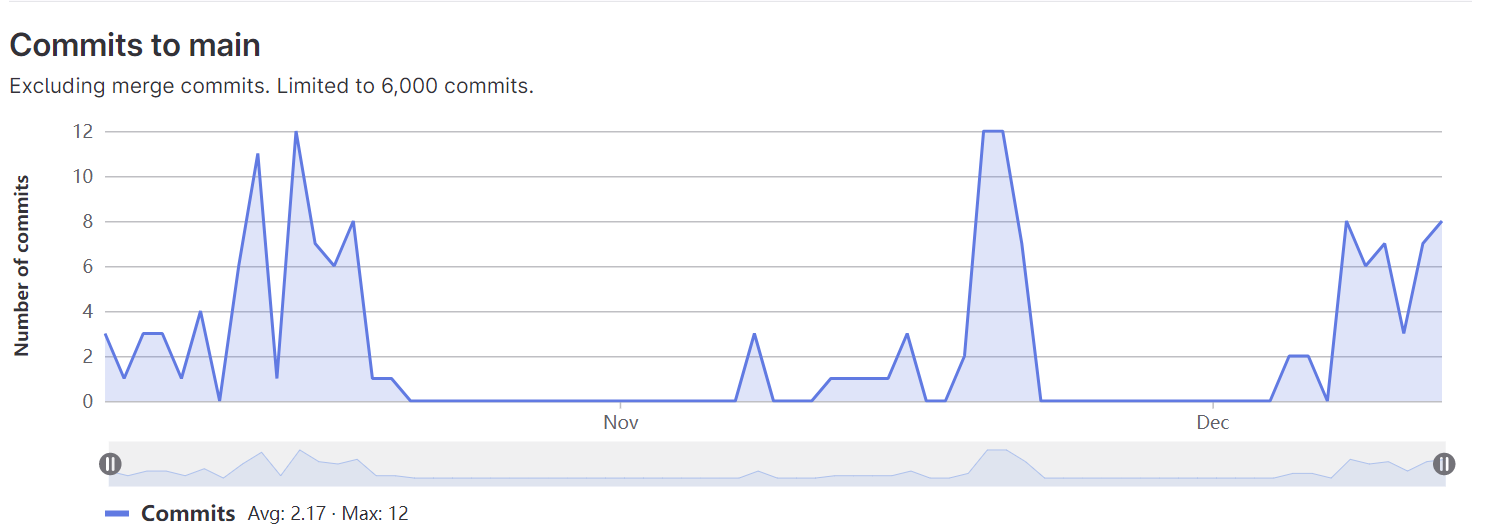
\includegraphics[scale=0.3]{slike/commits1.PNG} %veličina slike u odnosu na originalnu datoteku i pozicija slike
			\centering
			\label{}
		\end{figure}
	
	\begin{figure}[H]
		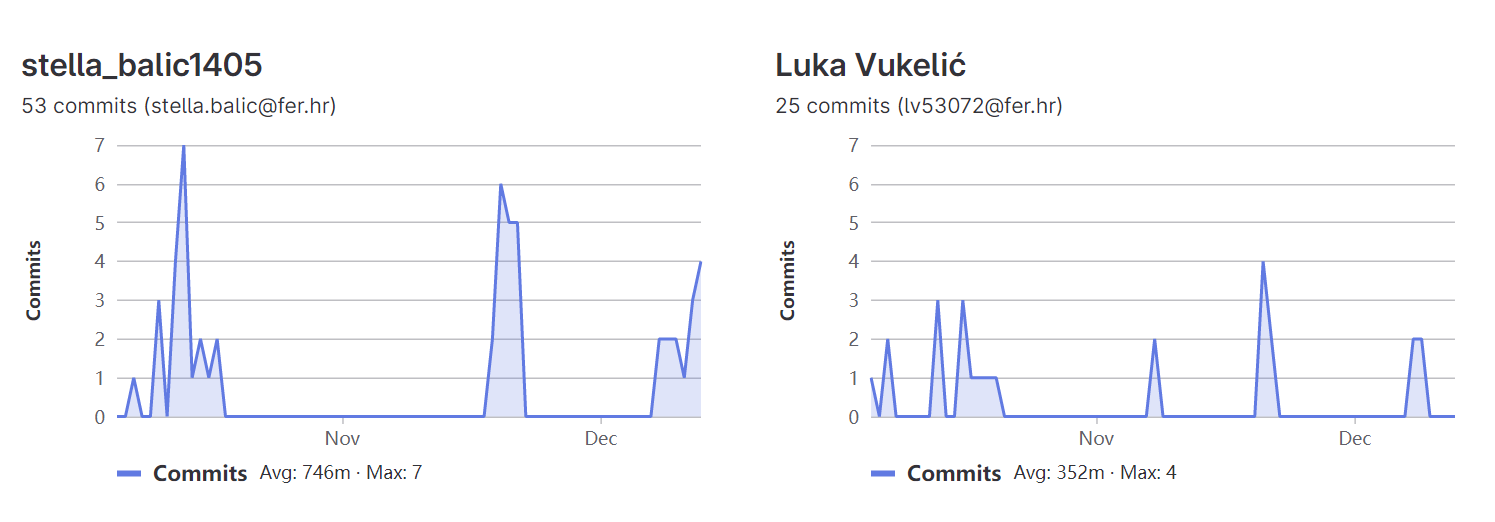
\includegraphics[scale=0.3]{slike/commits2.PNG} %veličina slike u odnosu na originalnu datoteku i pozicija slike
		\centering
		\label{}
	\end{figure}
   \begin{figure}[H]
	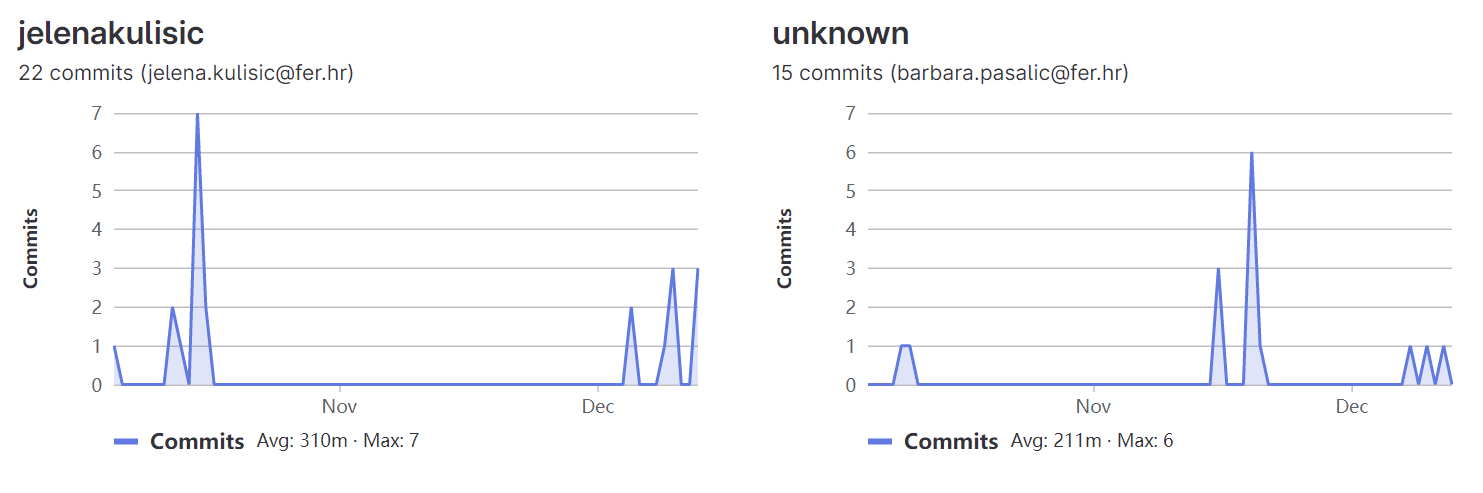
\includegraphics[scale=0.3]{slike/commits3.PNG} %veličina slike u odnosu na originalnu datoteku i pozicija slike
	\centering
	\label{}
\end{figure}
\begin{figure}[H]
	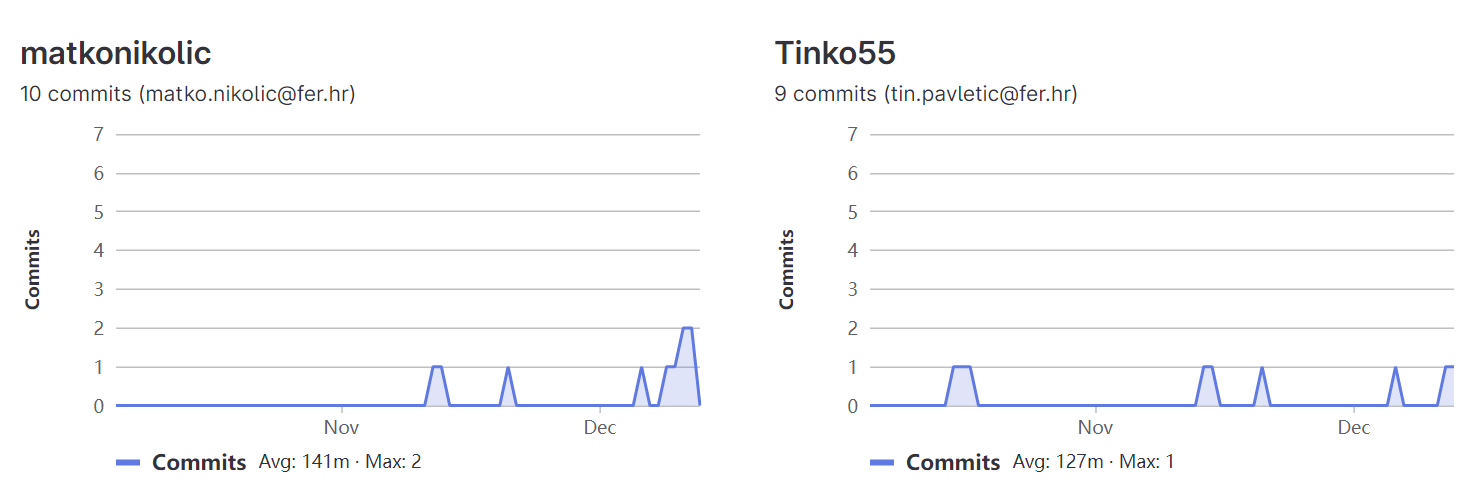
\includegraphics[scale=0.3]{slike/commits4.PNG} %veličina slike u odnosu na originalnu datoteku i pozicija slike
	\centering
	\label{}
\end{figure}
\begin{figure}[H]
	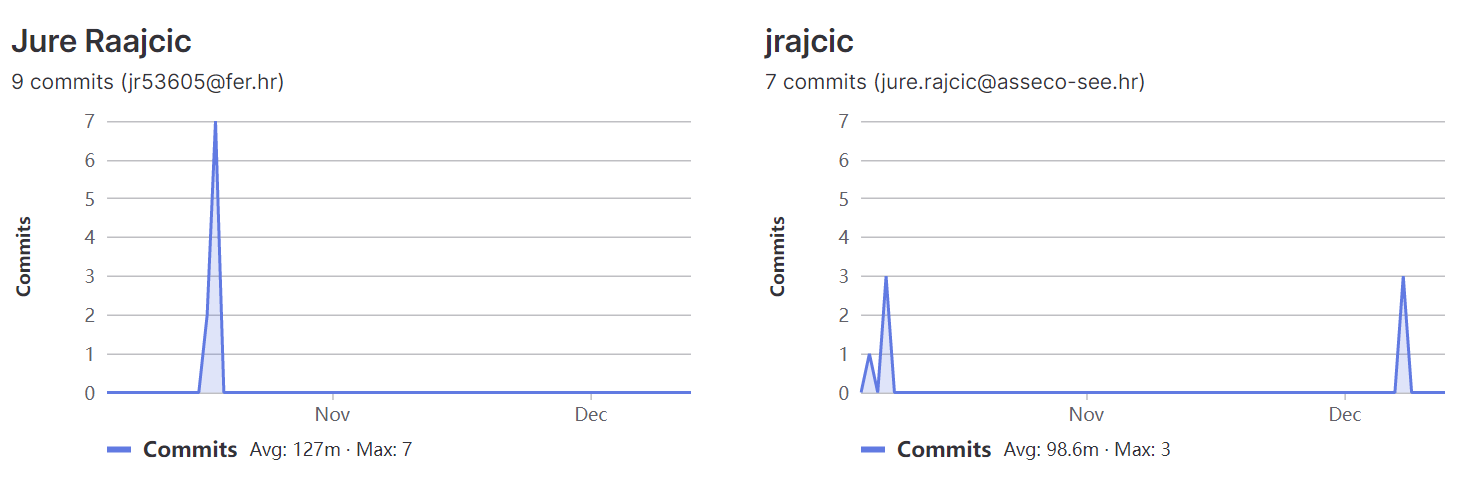
\includegraphics[scale=0.3]{slike/commits5.PNG} %veličina slike u odnosu na originalnu datoteku i pozicija slike
	\centering
	\label{}
\end{figure}
		
	


\end{document} %naredbe i tekst nakon ove naredbe ne ulaze u izgrađen dokument 


